\documentclass[USenglish]{article}

%\usepackage[utf8]{inputenc}
\RequirePackage[no-math]{fontspec}

\usepackage[small]{dgruyter}
\usepackage{microtype}
\usepackage{enumerate}
\usepackage{eqnarray}
\usepackage{colortbl}

\newcommand{\wrt}{w.\,r.\,t.\ }
\newcommand{\Wrt}{W.\,r.\,t.\ }
\newcommand{\eg}{e.\,g.,}
\newcommand{\Eg}{E.\,g.,}
\newcommand{\ie}{i.\,e.,}
\newcommand{\Ie}{I.\,e.,}
\newcommand{\Sub}[1]{\ensuremath{\mathrm{_{#1}}}}
\newcommand{\Sup}[1]{\ensuremath{\mathrm{^{#1}}}}
\newcommand{\Subsf}[1]{\ensuremath{\mathsf{_{#1}}}}
\newcommand{\Supsf}[1]{\ensuremath{\mathsf{^{#1}}}}
\newcommand{\pPB}{p\Subsf{PB}}
\newcommand{\mpPB}{\ensuremath{p_{\text{PB}}}}

\newcommand{\NACb}{NAC\Sub{bare}}
\newcommand{\NACa}{NAC\Sub{adj}}
\newcommand{\PGCd}{PGC\Sub{det}}
\newcommand{\PGCa}{PGC\Sub{adj}}

\newcommand*\Rot{\rotatebox{75}}

\definecolor{lg}{rgb}{.8,.8,.8}
\newcommand{\Dim}{\cellcolor{lg}}

\usepackage{gb4e-}

\usepackage{bbding}
\newcommand{\CheckIt}{\CheckmarkBold}
\newcommand{\CrossIt}{\XSolidBold}


\usepackage{natbib}
\bibliographystyle{./unified}

\begin{document}

  %\articletype{...}

  \author*[1]{Roland Schäfer}
  %\runningauthor{...}
  \affil[1]{Freie Universität Berlin}
  \title{Competing Constructions for German Measure Noun Phrases: from Usage Data to Experiment}
  \runningtitle{Competing Constructions for German Measure Noun Phrases}
  %\subtitle{...}
  \abstract{}
  \keywords{corpus methods and experimental methods, self-paced reading, forced-choice, alternations, hierarchical models, measure constructions, German}
  %\classification[PACS]{...}
  %\communicated{...}
  %\dedication{...}
  %\received{...}
  %\accepted{...}
  \journalname{(submitted)}
  \journalyear{2017}
  %\journalvolume{...}
  %\journalissue{...}
  %\startpage{...}
  %\aop
  %\DOI{...}


  
\maketitle



%%%%%%%%%%%%%%%%%%%%%%%%%%%%%%%%%%%%%%%%%%%%%%%%%%%%%%%%%%%%%%%%%%%%%%%
%%%%%%%%%%%%%%%%%%%%%%%%%%%%%%%%%%%%%%%%%%%%%%%%%%%%%%%%%%%%%%%%%%%%%%%
%%%%%%%%%%%%%%%%%%%%%%%%%%%%%%%%%%%%%%%%%%%%%%%%%%%%%%%%%%%%%%%%%%%%%%%


\section{Cognitively oriented corpus linguistics}
\label{sec:cogocl}

\subsection{Corpora, cognition, and alternations}

This paper deals with a morpho-syntactic alternation between two constructions that occurs only in a very specific type of measure noun phrase in German.
By \textit{alternation} I refer to a situation where two or more forms or constructions are available with no clear difference in acceptability, function, or meaning.
The study of alternations has a now longstanding tradition in cognitively oriented corpus linguistics (\citealp{BresnanEa2007,BresnanHay2010,BresnanFord2010,DivjakArppe2013,Gries2015,NessetJanda2010}, to name just a few publications).
This strand of research is based on the assumption that language is a probabilistic phenomenon \citep{Bresnan2007}, and choices of variants are neither chosen deterministically nor fully at random.
Instead, multifactorial models are constructed, which incorporate influencing factors from diverse levels, including contextual ones.
The estimation of the model quantifies the influence the factors have on the probability that either variant is chosen.

For such probabilistic generalisations estimated on corpus data, there has always been an interest in correlating the results with results from experimental work (for example, \citealp{ArppeJaervikivi2007,BresnanEa2007,BresnanFord2010,DivjakGries2008,DivjakEa2016,FordBresnan2013}).
This often called a \textit{validation} of the corpus-derived findings, but \citet[303]{Divjak2016a} criticises this choice of words \textit{because it creates the impression that behavioral experimental data is inherently more valuable than textual data}, citing \cite{TummersEa2005}, who state that a corpus is \textit{a sample of spontaneous language use that is} (\textit{generally}) \textit{realized by native speakers}.
This position, which I adopt, does not, however, imply that we can in some way \textit{deduce mental representations from patterns of use}, \ie\ from corpus data \citep[486--487]{Dabrowska2016}.%
\footnote{I suggest that the word \textit{induce} would be more appropriate than \textit{deduce}.}
In fact, it would be surprising if we could!
Nobody assumes that we can induce mental representations from experiments, which -- as opposed to corpus studies -- even provide a direct access to the cognitive agent and offer much better options to control and experimental conditions and nuisance variables.
Instead, a theory of cognitive representation is pre-specified, and predictions are derived from this theory \textit{before} the experiment or the corpus study is conducted.
Technical problems of statistical inference aside (see also Section~\ref{sec:rightstatistics}), a successful experiment corroborates the theory, and a failed experiment weakens the theory.
The simplest assumption would be that the same approach is adequate for corpus studies.

That said, the present study is conducted within the general paradigm of cognitive corpus linguistics and includes a comparison of the corpus findings with results from two experiments.
As a theoretical framework, I assume a model of similarity-based classification in the form of Prototype Theory.
Protoype Theory has been used in alternation research in cognitively oriented corpus linguistics, see \cite{DivjakArppe2013,Gries2003}.
It is assumed that the variables annotated in a corpus study on an alternation phenomenon define prototypes for the alternating variants.
The similarity of a given feature vector (in a concrete sentence where one of the variants is used) determines to a large extent which variant is chosen by speakers.
This entails that a variant of Prototype Theory with \textit{features} is assumed \citep{Rosch1978}, instead of the monolithic prototypes assumed in earlier versions.
While Prototype Theory is well suited for modeling constructional choices, it is just one similarity-based framework, the most prominent other framework being Exemplar Theory (\citealp{MedinSchaffer1978,Hintzman1986}; see \citealp{StormsEa2000} for a comparison of the theories in experimental settings).
Prototype Theory and Exemplar Theory differ mainly in whether they assume higher-level abstractions as part of the cognitive representation (Prototype Theory) or not (Exemplar Theory).
I am sceptical that corpus analysis alone could ever decide which theory is more adequate, given that substantial doubt has been voiced whether even experimental methods are ultimately able to do so \citep{Barsalou1990}.%
\footnote{In \cite{DivjakArppe2013}, a fruitful attempt was made to show how both models form a converging picture based on corpus data.}
Prototype Theory (with feature abstractions) is simply preferred here because it fits the established alternation modeling paradigm, which relies on features being weighted (in a sense) in statistical models.
In Section~\ref{sec:analyses}, a prototype-theoretical parlance is therefore adopted.

Before moving on to the description of the phenomenon and the corpus study in Sections~\ref{sec:descriptive} and \ref{sec:analyses}, I comment on the statistical methods used in the corpus study in Section~\ref{sec:rightstatistics} because the discussion is closely related to basic questions of the cognitive approach in corpus linguistics.


%%%%%%%%%%%%%%%%%%%%%%%%%%%%%%%%%%%%%%%%%%%%%%%%%%%%%%%%%%%%%%%%%%%%%%%
%%%%%%%%%%%%%%%%%%%%%%%%%%%%%%%%%%%%%%%%%%%%%%%%%%%%%%%%%%%%%%%%%%%%%%%

\subsection{On statistical analysis}
\label{sec:rightstatistics}

In this section, I motivate the choice of statistical models which I use later in Section~\ref{sec:corpusstudies}.
Readers might think that the method used here for modeling grammatical alternations -- namely (Hierarchical) Logistic Regression\slash Generalised Linear (Mixed) Models or GLM(M)s -- does not require much motivation.
After all, GLMMs have been established as the major tool in the analysis of alternation phenomena.
All studies mentioned at the outset of Section~\ref{sec:cogocl} use GLM(M)s \citep{BresnanEa2007,BresnanHay2010,BresnanFord2010,DivjakArppe2013,Gries2015,NessetJanda2010} use some form of regression\slash GLM(M).
Over the past few years, however, modified or alternative methods have been proposed.
From among these methods, I just make a few remarks on Bayesian estimation (see \citealp{GelmanEa2014}), as it was proposed in \cite{Levshina2016,Divjak2016a}, for example.
Conceptually, I see three points of discussion that should be kept apart.
First, Bayesian methods are sometimes touted as superior tools for scientific inference compared to frequentist methods.
Second, it has been proposed that the Bayesian interpretation of probability is more cognitively adequate for the modeling of linguistic data.
Third, and very specific to this paper, given established methods in the modeling of alternation and variation, it has to be decided whether so-called Bayesian methods lead to substantially different results.

As for the first question, this is not quite the place to discuss it fully.
The basic distinction is a philosophical one and related to the concepts of \textit{direct} and \textit{inverse probability} (\eg\ \citealp{Senn2011}).
Frequentists assume that models and parameters are fixed, for example a model specifying that a coin is fair.
We can then calculate for observed data (for example a measurement of $3$ heads in an experiment with $10$ tosses) how often such a result or a more extreme result would occur if the model were true and we repeated the experiment arbitrarily often.
This is essentially the frequentist notion of direct probability, \ie\ long-run frequencies under replication.
Standard tests in the Fisher and Neyman-Pearson traditions as well as Neyman confidence intervals are based on this concept of probability.
Bayesian approaches (in the now common interpretation), on the other hand, condition on the particular data and quantify inductively the probability of model parameters given the data.
The parameters are thus not fixed, and the probability is usually equated with researchers' posterior beliefs about model parameters.
There is actually a debate among Bayesians about the proper interpretation of Bayesian methods, and whether a notion of hypothesis testing is compatible (or even already contained) in the Bayesian approach.
In \citet[10]{GelmanShalizi2013}, the authors -- prominent Bayesians themselves -- acknowledge that a theory of testing is a desideratum, and they state about the standard inductive interpretation of Bayesianism that \textit{most of this received view of Bayesian inference is wrong}, and they develop a Bayesian notion of $p$ values (see also \citealp{Mayo2013}, for a frequentist reply; also \citealp{Senn2011} on different strands of Bayesianism and their stance on inductive vs.\ deductive reasoning).
Clearly, in such quarrels between and among camps of philosophers of science and statisticians it is difficult for mere practitioners to take sides.

These quarrels relate to the second question, however.
\citet[301--302]{Divjak2016a} speaks favourably of Bayesian methods because the Bayesian concept of probability is more adequate for cognitive modeling compared to the frequentist one.
Her argument is part of a larger body of literature asking for cognitively plausible modeling techniques, for example Naive Discriminative Learning (NDL; \citealp{Baayen2011,BaayenEa2013,MilinEa2016,TheijssenEa2013}). 
On p.\ 303 of \cite{Divjak2016a}, the author goes on to explicitly mention NDL.
Yet, neither frequentist nor Bayesian methods were conceived as cognitive models, but as systems of inference for scientists (see above, and see also \citealp[302]{Divjak2016a}).
The fundamental question that lurks behind such arguments is how we interpret our statistical models (estimated on corpus data).
Are they inductive models of cognitive representations that also human learners would infer from being exposed to the corpus data?%
\footnote{In which case we are doing \textit{data science in language research} in the words of \citealp{MilinEa2016}.}
Or are they tests of theories that are pre-specified and merely tested for predictive accuracy on linguistic output data contained in corpora.
In the former case, we adopt a strong \textit{corpus as input} hypothesis and should definitely resort to methods like NDL.
However, this would most likely require us to toss most previous work done in (cognitive) linguistics into the bin and abandoning all high-level generalisations that most existing studies have been based upon.
In fact, arguments to this extreme effect and against using high-level generalisation have been made, for example in \cite{BaayenEa2016}, \citet[299--300]{Divjak2016a}, \cite{RamscarPort2016}, \cite{TheijssenEa2013}.
In the latter and less extreme case, the cognitive commitment does, however, not necessarily extend to the statistical methods used.
These methods then do not need to be any more cognitively plausible than an ANOVA used to analyse the results from an experiment.
I view my own work (see Sections~\ref{sec:germanmeasurenps}--\ref{sec:experimental}) in the tradition of testing theories that embrace high-level generalisations, and I agree to provisionally use Likelihood methods (see below).
I remain fully agnostic with respect to the question which approach is `right'.
The best strategy for cognitive linguistics as a field might be to cultivate many methods while making sure that each method is applied carefully and competently.

The third point, then, is the most practically relevant in the context of this paper.
In her otherwise excellent study, \citet[251--252]{Levshina2016} argues for Bayesian estimation in mixed regression settings.
First, she claims that \textit{while frequentist statistics only allows one to test whether the null hypothesis can be rejected, Bayesian statistics enables one both to test the null hypothesis and to estimate the probability of specific parameter values given the data}.
This does not do justice to frequentist methods in that mere rejection of the null hypothesis is characteristic only of Fisher's approach, but in the Neyman-Pearson approach, results ideally \textit{favour} the main hypothesis vis-à-vis the alternative hypothesis (cf.\ \citealp{Lehmann1993,Lehmann2011,Perezgonzalez2015}).
Also, especially Neyman-style frequentism has well-known extensions to estimation (see \citealp{GreenlandEa2016}, esp.\ p.\ 340).
She then explains that a \textit{distinctive feature of Bayesian statistics is the use of so-called priors} and that \textit{posterior probabilities depend on both the prior beliefs and the data, whereas the results of a frequentist model depend only on the data} \cite[252]{Levshina2016}.
Remarkably, given this statement, she does \textit{not} use informative priors, and in her footnote 8 \cite[252]{Levshina2016} admits that priors were probed using trial and error.
So, the proclaimed major advantage of Bayesian modeling was apparently not taken advantage of.%
\footnote{In the words of \cite{Senn2011}: \textit{You may believe you are a Bayesian but you are probably wrong}.
\citet[347--348]{GelmanHill2006} \textit{view any noninformative prior distribution as inherently provisional} and give recommendations how to proceed once posteriors have been obtained from noninformative priors.}
Now, Maximum Likelihood Estimation (MLE) -- the traditional method which could have been used instead -- is not exactly \textit{frequentist} in the sense of Neyman-Pearson testing theory.
MLE, like inductive Bayesianism, conditions on the data in as much as it searches for the most likely set of parameters given the particular data.
What is more, Bayesian estimators are in fact based the Likelihood function and merely multiply it by the prior \citep[6--8]{GelmanEa2014}.
If the prior is flat, results converge (see also \citealp[347]{GelmanHill2006}).
The same is true if the sample size is large compared to the number of parameters, at least for finite-dimensional models \citep[1119--1120]{Freedman1999}, a well-established result known as the Bernstein-von Mises theorem.
With a modest model structure including $17$ fixed effects and $2,646$ data points in \cite{Levshina2016}, it is highly likely that the same results would have obtained with Maximum Likelihood methods.
In fact, she admits that changing the priors did not lead to substantially different results in her footnote 8.
This is a clear sign that the prior is \textit{swamped} by the data \citep[1119]{Freedman1999}.
Going back to the argument that Bayesian methods are allegedly more cognitively plausible than `frequentist' methods, the claim might still be true.
However, most similar studies (back to \citealp{BresnanEa2007}) use an estimator (MLE) that is not frequentist, and as cognitively plausible as Bayesian estimators because it most likely produces the same results in these studies.
If for Levshina's study, results from Bayesian and MLE methods did, in fact, \textit{not} converge, it would have been an ideal occasion to demonstrate the superiority of the algorithms used in Bayesian estimation.
After all, there are situations where Bayesian estimators can be more robust, namely with heavily censored data, complex hierarchical models, perfect separation, etc. (see \citealp{Freedman1999}, \citealp[345--348]{GelmanHill2006}).
I want to reiterate that these points do not in any way invalidate the results presented in \cite{Levshina2016}.
However, being \textit{Bayesian} is most likely not among its selling points.
That said, I want to voice the concern that probably many practitioners are already struggling with getting an adequate grasp of advanced statistical methods, and that it might therefore be wise to use the more conservative and better understood method if the alternative method is not absolutely required for substantive reasons.
In Section~\ref{sec:corpushierarchicalmodel}, I compare my own hierarchical models estimated with Bayesian and MLE estimators to demonstrate their expectable convergence.

This concludes the general introduction.
In the remainder of the paper, I introduce the alternation phenomenon (Section~\ref{sec:descriptive}) and suggest a theory-driven set of factors influencing the alternation (Section~\ref{sec:analyses}).
Then, the corpus study is presented including an appropriate statistical analysis (Section~\ref{sec:corpusstudies}).
The two experiments which correlate results from the corpus study with experimental results are then reported (Section~\ref{sec:experimental}) before I sum up the paper in Section~\ref{sec:conclusion}.


%%%%%%%%%%%%%%%%%%%%%%%%%%%%%%%%%%%%%%%%%%%%%%%%%%%%%%%%%%%%%%%%%%%%%%%
%%%%%%%%%%%%%%%%%%%%%%%%%%%%%%%%%%%%%%%%%%%%%%%%%%%%%%%%%%%%%%%%%%%%%%%
%%%%%%%%%%%%%%%%%%%%%%%%%%%%%%%%%%%%%%%%%%%%%%%%%%%%%%%%%%%%%%%%%%%%%%%


\section{Case assignment in German measure NPs}
\label{sec:germanmeasurenps}


\subsection{Two stable cases and a case alternation}
\label{sec:descriptive}

In this section, I introduce and illustrate the relevant alternating constructions.
I describe the narrowly defined syntactic configuration in which the alternation occurs, and I motivate the focus on \textit{only} this narrow range rather than, for example, the whole range of nominal constructions expressing quantities.

I use the term \textit{measure noun phrase} (MNP) to refer a noun phrase (NP) in which a kind-denoting (count or mass) noun depends on another noun that specifies a quantity of the objects or the substance denoted by the kind noun.
I call the kind-denoting noun simply the \textit{kind noun} and the quantity-denoting noun the \textit{measure noun}.
For illustration purposes, in the English \textit{a cup of fine coffee}, \textit{cup} is the measure noun, and \textit{coffee} is the kind noun.
Measure nouns can be all sorts of nouns which genuinely denote a quantity (such as \textit{litre} or \textit{amount}) but also nouns denoting containers, collections, etc. (such as \textit{glass} or \textit{bucket}).
In a similar vein, \citet[284]{Brems2003} considers nouns as measure nouns \textit{which, strictly speaking, do not designate a `measure', but display a more nebulous} (\textit{sic!}) \textit{potential for quantification} (see also \citealp[530]{Koptjevskaja2001}, and \citealp[338]{Rutkowski2007}).

In the case at hand, three different syntactic configurations need to be distinguished \wrt case assignment inside German measure noun phrases.
If the kind noun forms an NP with a determiner, the construction resembles (and is usually called) a \textit{pseudo-partitive} (on partitives and pseudo-partitives see, e.\,g., \citealp{Barker1998,Selkirk1977,Stickney2007,Vos1999}; for a recent application of the terminology to German, see \citealp{Gerstenberger2015}).%
\footnote{If the kind noun is definite, the construction instantiates a true partitive.
Whereas partitives are constructions denoting a proper part-of relation as in \textit{a sip of the wine}, pseudo partitives -- albeit syntactically similar and diachronically related to partitives in many languages -- merely denote quantities and contain indefinite kind nouns as in \textit{a sip of wine}.%
In the literature on German, some authors incorrectly call the pseudo-partitive a \textit{partitive} \cite{Hentschel1993} while some realise the difference and at least mention it \citep{Eschenbach1994,GallmannLindauer1994,Loebel1989,Zimmer2015}.
}
Here, the kind noun is in the genitive, and I refer to the construction in (\ref{ex:intro:pseudopartitive1}) as the \textit{Pseudo-partitive Genitive Construction} (PGC).

\begin{exe}
%  \ex\label{ex:intro:pseudopartitive}
%  \begin{xlist}
    \ex[ ]{\label{ex:intro:pseudopartitive1}\gll Wir trinken [[eine Tasse]\Sub{Acc} [eines leckeren Kaffees]\Sub{Gen}]\Sub{Acc}.\\
    we drink a cup a tasty coffee\\
    \glt We drink a cup of a tasty coffee.}
%    \ex[*]{\label{ex:intro:pseudopartitive2} Wir trinken [[eine Tasse]\Sub{Acc} [einen leckeren Kaffee]\Sub{Acc}]\Sub{Acc}.}
%  \end{xlist}
\end{exe}

If the kind noun is bare -- \ie\ if it does neither come with a determiner nor a modifying adjective -- it has to agree in case with the measure noun, and the genitive seen in the PGC is not acceptable, see (\ref{ex:intro:narrowapposition2}).

\begin{exe}
%  \ex\label{ex:intro:narrowapposition}
%  \begin{xlist}
%    \ex[*]{\label{ex:intro:narrowapposition1} Wir trinken [[eine Tasse]\Sub{Acc} [Kaffees]\Sub{Gen}]\Sub{Acc}.}
    \ex[ ]{\label{ex:intro:narrowapposition2}\gll Wir trinken [[eine Tasse]\Sub{Acc} [Kaffee]\Sub{Acc}]\Sub{Acc}.\\
    we drink a cup coffee\\
    \glt We drink a cup of coffee.}
%  \end{xlist}
\end{exe}

This construction is usually classified as a \textit{Narrow Apposition Construction} \citep{Loebel1986}, henceforth NAC.%
\footnote{The construction as in (\ref{ex:intro:narrowapposition2}) is also referred to as the \textit{Direct Partitive Construction} for other Germanic languages in which the PGC with the synthetic genitive is not available.
This nomenclature makes sense in contrast to the \textit{Indirect Partitive Construction} with prepositional linkers translating to `of' -- \ie\ analytic genitives -- in such languages, see \cite{HankamerMikkelsen2008} for Danish.
For German, this terminology is not distinctive enough, which is why I use the terms NAC and PGC.}
Notice that the unavailability of the genitive on the kind noun can be seen as following from a rather quirky constraint that genitive NPs in German require the presence of some strongly case-marked element (determiner or adjective) in addition to the head noun in order to be acceptable (\citealp{GallmannLindauer1994,Schachtl1989}; see also \citealp[160]{Eisenberg2013b}).
While only an accusative is shown in (\ref{ex:intro:narrowapposition2}), the kind noun obligatory agrees in case also with nominative and dative measure nouns.

The actual alternation can be observed \textit{only when the kind noun occurs with an attributive adjective but without a determiner}, as in (\ref{ex:intro:alternation}), where both the NAC in (\ref{ex:intro:alternation1}) and the PGC in (\ref{ex:intro:alternation2}) are equally acceptable.
They are by-and-large functionally and semantically equivalent.
However, Section~\ref{sec:analyses} is devoted to developing hypotheses about subtle differences between them.%
\footnote{Some descriptive and normative grammars take stronger positions w.\,r.\,t.\ the acceptability of the two options.
See \cite{Hentschel1993,Zimmer2015} for analyses of the sometimes absurd stances taken in grammars of German.
As the usage and experimental data presented below (especially Section~\ref{sec:exp:fc}) should render it clear, there might be preferences under certain circumstances, but we cannot assume either construction to be unacceptable.
}

\begin{exe}
  \ex\label{ex:intro:alternation}
  \begin{xlist}
    \ex[ ]{\label{ex:intro:alternation1}\gll Wir trinken [[eine Tasse]\Sub{Acc} [heißen Kaffee]\Sub{Acc}]\Sub{Acc}.\\
    we drink a cup hot coffee\\
    \glt We drink a cup of hot coffee.}
    \ex[ ]{\label{ex:intro:alternation2} Wir trinken [[eine Tasse]\Sub{Acc} [heißen Kaffees]\Sub{Gen}]\Sub{Acc}.}
  \end{xlist}
\end{exe}

\begin{table}
  \centering
  \begin{tabular}{lccc}
    \multicolumn{1}{r}{kind NP is:} & bare noun NP & NP with adjective & NP with determiner \\
    & [\ldots N\Subsf{meas} [N\Subsf{kind}]] & [\ldots N\Subsf{meas} [AP N\Subsf{kind}]] & [\ldots N\Subsf{meas} [D N\Subsf{kind}]] \\
    \midrule
    narrow apposition         & \NACb & \NACa & ---   \\
    pseudo-partitive genitive & ---   & \PGCa & \PGCd \\
  \end{tabular}
  \caption{Distribution of the NAC and PGC constructions in different NP structures}
  \label{tab:constructions}
\end{table}

The distribution of the case patterns in the NAC (case identity between the measure noun and the kind noun) and in the PGC (genitive on the kind noun, regardless of the case of the measure noun) depending on the structure of the kind NP are summarised in Table~\ref{tab:constructions}.
I call the narrow apposition construction with a bare kind noun the \NACb, the partitive genitive with a determiner in the kind noun phrase the \PGCd.
I call the alternating variants with an adjective but no determiner in the kind noun phrase \NACa, and \PGCa, respectively.
This paper is about the middle column of Table~\ref{tab:constructions}, \ie\ the syntactic configuration in which two different case patterns are acceptable.

I now turn to some more subtle issues related to the measure noun case alternation, namely:

\begin{enumerate}[i.]
  \item{\label{it:intro:idiot} alleged alternatives to the \NACa\ and the \PGCa}
%  \item{\label{it:intro:datsg} alternative \textit{weak} forms of dative singular neuter adjectives}
%  \item{\label{it:intro:femsg} case syncretism in feminine NPs}
  \item{\label{it:intro:plurl} similar constructions with plural/collective kind nouns}
  \item{\label{it:intro:noifl} grammaticalised non-inflected measure nouns}
  \item{\label{it:intro:other} alternative constructions for expressing quantities}
\end{enumerate}

\vspace{-1\baselineskip}

First of all, (\ref{it:intro:idiot}) refers to claims found in some grammars that a generic nominative, accusative, and even dative on the kind noun are used instead of the genitive (\PGCa) or case agreement (\NACa).
Overviews can be found in \citealp{Hentschel1993,Zimmer2015}, and (\ref{ex:intro:gennom}) shows a putative generic nominative on the kind noun inside an accusative MNP.

\begin{exe}
    \ex[*]{\label{ex:intro:gennom} Wir trinken [[eine Tasse]\Sub{Acc} [heißer Kaffee]\Sub{Nom}]\Sub{Acc}.}
\end{exe}

It was shown empirically in \cite{Hentschel1993} that such variants are de facto not acceptable.
Also, in my corpus sample, they simply did not occur.
Even if they are accepted by some speakers, their extremely low frequency makes it virtually impossible to study them using either corpus methods (Section~\ref{sec:corpusstudies}), and I consequently ignore them.

% As for (\ref{it:intro:datsg}), a complication with neuter kind nouns in the dative is mentioned by \citet[20--22]{Zimmer2015}.
% In the \NACa, the adjective normally inflects with the so-called \textit{strong} case and number suffixes, which are used when no determiner with strong inflection is present in the NP.
% \cite{Zimmer2015} reports a high number of occurrences of adjectives being inflected with the \textit{weak} inflectional marker, which are normally only used if a strongly inflected determiner precedes the adjective: \textit{kalt-en Wasser} `cold water' instead of \textit{kalt-em Wasser}.%
% \footnote{See Section~\ref{sec:analyses} for more discussion of adjectival inflection.}
% In my corpus sample, this tendency was not nearly as clear, and there was a high number of very noisy sentences among those potentially showing this pattern.
% Hence, I do not discuss these forms.%
% \footnote{All corpus data and scripts used for this paper will be released freely, so further examination of the few cases maybe showing this kind of inflection is possible.}
% 
% \label{page:femininesyncretism}
% With feminine kind nouns, (\ref{it:intro:femsg}) is relevant.
% Whereas the singular masculine and neuter nominal subsystem is a four case system (at least for NPs with adjectives and determiners), feminine singular NPs show nominative-accusative and dative-genitive syncretisms.
% Table~\ref{tab:syncretisms} shows this as well as the partial syncretism in the plural, where no gender distinctions are made.
% This means that with dative measure nouns, the alternation is unobservable if the kind noun is feminine, and it is problematic to speak of a \textit{genitive} kind noun construction in this case.
% This is taken into account in the statistical modeling and the discussion presented in Section~\ref{sec:corpusstudies}.
% 
% \begin{table}
%   \centering
%   \begin{tabular}{llll}
%      & Masculine\slash Neuter & Feminine & Plural \\
%      \midrule
%      nominative & rot-er Wein    & \multirow{2}{*}{frisch-e Sahne}   & \multirow{2}{*}{klein-e Äpfel} \\
%      accusative & rot-en Wein    &                                   &                                \\
%      dative     & rot-em Wein    & \multirow{2}{*}{frisch-er Sahne}  & klein-en Äpfel-n               \\
%      genitive   & rot-en Wein-es &                                   & klein-er Äpfel                 \\
%   \end{tabular}
%   \caption{Case syncretisms in NPs with an adjective and without a determiner (\textit{roter Wein} `red wine', \textit{frische Sahne} `fresh cream', \textit{kleine Äpfel} `small apples')}
%   \label{tab:syncretisms}
% \end{table}

Turning to (\ref{it:intro:plurl}), readers might have noticed that so far only MNPs denoting quantities of substances (mass kind nouns such as \textit{ein Glas roter Wein\slash roten Weines} `a glass of red wine') have been discussed.
If the kind noun is a plural count noun as in \textit{ein Sack kleine Äpfel} (\NACa) or \textit{ein Sack kleiner Äpfel} (\PGCa) `a bag of small apples', a similar alternation between PGC and NAC can be observed.
In line with experimental results reported in \citet[15--16]{Zimmer2015}, I found that the PGC is so dominant with plural kind nouns (67 of 861 cases or over 92\%, cf.\ Section~\ref{sec:corpusstudies}) that the alternation cannot be analysed in the same way as in the singular case.%
\footnote{More concretely, if these cases were included in the regression analysis of the corpus data along with a factor encoding the number of the kind noun, this factor would most assuredly override any other regressor for the data points with a plural kind noun.}
While this will play a role in the interpretation of the corpus findings, MNPs with plural kind nouns will not be included in the corpus study and the experiments reported here.

As for (\ref{it:intro:noifl}), some measure nouns have been grammaticalised in a way that they always appear non-inflected.
They are typical measure nouns like \textit{Gramm} `gram', \textit{Pfund} `pound' or \textit{Prozent} `percent', which do not have plural forms at all.
%\footnote{With neglectable frequency, this effect is extended to container nouns like \textit{Glas} `glass', but with a twist.
%A non-inflected variant \textit{zwei Glas roter Wein} `two glasses of wine' and an inflected variant \textit{zwei Gläser roter Wein} co-exist.
%The non-inflected variant denotes the quantity of wine fitting into two glasses, the inflected variant denotes two glasses filled with wine.}
I treat these cases like other measure nouns because they enter into both the \NACa\ as in (\ref{ex:uninflectedmeasures:a}) and the \PGCa\ as in (\ref{ex:uninflectedmeasures:b}).
In Section~\ref{sec:analyses}, degrees of grammaticalisation as a factor influencing the alternation will be discussed, however. 

\begin{exe}
  \ex\label{ex:uninflectedmeasures}
  \begin{xlist}
    \ex{\label{ex:uninflectedmeasures:a} zwei Gramm brauner Zucker}
    \ex{\label{ex:uninflectedmeasures:b}\gll zwei Gramm braunen Zuckers\\
                                         two gram brown sugar\\
				         two grams of brown sugar}
  \end{xlist}
\end{exe}

Finally, (\ref{it:intro:other}) suggests that there are alternative ways of expressing similar quantificational meanings.
In the variationist tradition, which is strongly influenced by Labovian sociolinguistics, the \textit{principle of accountability} would dictate that proper studies should examine a variationist \textit{variable}, \ie\ all different \textit{ways of saying the same thing} (\citealp{Labov1966}, \citealp{Labov1969}, for an overview see \citealp{Tagliamonte2012}).
In the case at hand, the variable might be something like \textit{measuring quantities of substances and collections}.
I argue that it is fully justified to focus narrowly on \NACa\ and \PGCa\ with their well-defined morpho-syntactic properties, mostly because the alternative constructions are not used in the same range of contexts.
Two major alternatives might be considered.
First of all, the analytic (pseudo-)partitive with \textit{von} `of' is only available as an alternative to the PGC if the kind noun phrase contains a (definite or indefinite) determiner as in (\ref{ex:analyticalpartitive}).

\begin{exe}
  \ex\label{ex:analyticalpartitive} 
  \begin{xlist}
    \ex[ ]{\label{ex:analyticalpartitive:a}\gll ein Glas von dem roten Wein\\
                                                a glass of the red wine\\
                                                \glt a glass of the red wine
       }
    \ex[*]{\label{ex:analyticalpartitive:b}\gll ein Glas von rotem Wein\\
                                                a glass of red wine\\
                                                \glt a glass of red wine
       }
  \end{xlist}
\end{exe}

This means that the \textit{von} (pseudo-)partitive does not compete with the \NACa\ and the \PGCa.
In fact, there is not a single context in which they can be interchanged. 

Second, constructions with \textit{voll} (\textit{von})\slash\textit{voller} `full (of)' and \textit{mit} `with' are available, see (\ref{ex:alternatives}).

\begin{exe}
  \ex\label{ex:alternatives}
  \begin{xlist}
  \ex{\label{ex:voll}\gll   ein Glas voll von rotem Wein\\
                            a glass full of red wine\\
			    \glt a glass full of red wine}
  \ex{\label{ex:voller}\gll ein Glas {voll\slash voller} {rotem\slash roter} Wein\\
                            a glass full-of red wine\\
			    \glt a glass full of red wine}
  \ex{\label{ex:mit}\gll    ein Glas mit rotem Wein\\
                            a glass with red wine\\
			    \glt a glass with red wine in it\slash a glass filled with red wine}
  \end{xlist}
\end{exe}

These construction have very idiosyncratic properties (the construction with \textit{voller} is discussed in \citealp{Zeldes2018}, the construction with \textit{mit} is discussed in \citealp{Bhatt1990}), they are not semantically equivalent to the NAC and the PGC, and they are only available for a small subset of measure nouns.
All of these constructions are only used with measure nouns denoting containers, and the whole NP always refers to the container, and never to the quantity contained in it.
They are consequently incompatible with measure nouns denoting natural portions such as \textit{Schluck} `gulp' or \textit{Haufen} `heap' and strongly grammaticalised nouns such as \textit{Gramm} `gram'.
This disqualifies them as alternatives to the \NACa\ or \PGCa\ in most contexts, and they are thus decidedly \textit{not} more ways of saying the same thing. 
It is therefore reasonable to focus on the two well-defined variants.

This concludes the descriptive overview of the phenomenon.
I have shown that there is an alternation between two measure noun constructions in a narrow syntactic configuration (kind NP with an adjective but without a determiner), and that the two constructions differ in the case of the kind noun (case agreement with the measure noun or genitive).
I turn to some more theory-oriented discussion in the next section.


%%%%%%%%%%%%%%%%%%%%%%%%%%%%%%%%%%%%%%%%%%%%%%%%%%%%%%%%%%%%%%%%%%%%%%%
%%%%%%%%%%%%%%%%%%%%%%%%%%%%%%%%%%%%%%%%%%%%%%%%%%%%%%%%%%%%%%%%%%%%%%%

\subsection{Factors controlling the alternation}
\label{sec:analyses}

This section briefly reviews existing analyses of the \PGCa vs.\ \NACa\ alternation and related issues.
I also develop my own analysis and the appropriate hypotheses for the empirical studies presented in Sections~\ref{sec:corpusstudies} and \ref{sec:experimental}.
I discuss four main aspects:
first, the different syntactic structures of the variants \NACa\ and \PGCa\ in relation to their syntactic prototypes \NACb\ and \PGCd;
second, degrees of grammaticalisation of the measure noun associated with the two prototypes;
third, a semantic prototypicality effect of the degrees of grammaticalisation (a preference to occur with cardinals);
fourth, preferences in different registers.

% MORPHO-SYNTAX AND PROTOTYPES

My analysis is based on the idea that the relevant syntactic structure [N\Sub{1}~[A~N\Sub{2}]\Sub{NP\Sub{2}}]\Sub{NP\Sub{1}} as instantiated in the \NACa\ and the \PGCa\ is ambiguous.
To show this, the first question is which noun constitutes the head of the whole construction.
This was answered quite clearly by \cite{Loebel1986} already (see also \citealp[213]{Eschenbach1994}, and \citealp[16]{GallmannLindauer1994}).
Subject-verb agreement is always realised on the measure noun, and we can therefore assume that the measure noun is the head.
However, the MNP-internal structure has more interesting cues to offer if the strong\slash weak inflection patterns of adjectives are taken into account.
In NPs with a strongly inflected determiner, attributive adjectives inflect according to the massively syncretistic \textit{weak} pattern.
%\footnote{The weak pattern has only two suffixes.
%The structural cases (nominative and accusative) in the singular are marked with \textit{-e}, the oblique cases (dative and genitive) as well as the entire plural are marked with \textit{-en}.
%The only exception to this rule is the masculine accusative singular, which is also marked with \textit{-en}.}
If there is no determiner (as is the case in the alternating constructions), attributive adjectives inflect like determiners themselves, however.
This is called the \textit{strong} inflectional pattern.
Thus, the adjectives in the \NACa\ and the \PGCa\ have properties of adjectives as well as determiners.
On the one hand, they are lexical adjectives and function as attributive modifiers.
On the other hand, they are inflected like determiners, and they are the leftmost element in the NP, which is typical of determiners.
This unusual double nature of adjectives in NPs without determiners leads to a plausible probabilistic interpretation of the pattern shown in Table~\ref{tab:constructions}.
Whenever speakers classify the adjective in the kind noun phrase more as a determiner, they have to use the \PGCa\ because, if there is a determiner, the PGC is the only option.
When they classify the adjective more as an adjective, the kind NP has no determiner, and they have to use the \NACa.%
\footnote{While the generative analysis presented in \cite{Bhatt1990} cannot properly deal with probabilistic effects, Bhatt comes close to this interpretation by analysing the kind NP in the GPC as a DP and in the NAC as an NP.}

This morpho-syntactic ambiguity means that the \NACa\ is in fact a \NACb\ in disguise, and the \PGCa\ is a \PGCd\ in disguise.
This should ideally be reflected in the following basic selection effect:
It is known from frameworks like Collexeme Analysis \citep{GriesStefanowitsch2004} that lemmas are attracted with different strengths by competing constructions.
If the \NACa\ is highly similar to the \NACb\ and the \PGCa\ is highly similar to the \PGCd, the probability with which individual noun lemmas appear in the alternating constructions should be predictable at least partly from the relative frequency with which the same lemmas are used in the non-alternating constructions (see \citealp[246--249]{Levshina2016} for a similar idea in a different context).
Nouns which occur proportionally more often in the \PGCd\ should favour the \PGCa, and nouns which occur proportionally more often in the \NACb\ should favour the \NACa.
This basic attraction effect will be quantified in the corpus study Section~\ref{sec:corpusstudies}.

% GRAMMATICALISATION

In a probabilistic framework like Prototype Theory, the crucial question (beyond simple lemma preference effects) is, however, what controls speakers' decisions to use either variant. 
In the remainder of this section, I argue that the NAC and the PGC are prototypes associated with different degrees of the grammaticalisation of the measure noun, a related morpho-syntactic property, and register effects.
The degree of similarity of a given instance to either of the two prototypes makes speakers chose the \NACa\ or the \PGCa.
I first turn to grammaticalisation.
It is often assumed that pseudo-partitives arise as a form of grammaticalised partitives (\eg\ \citealp[536--539]{Koptjevskaja2001} for Finnish and Estonian, \citealp[559]{Koptjevskaja2001} for European languages per se).
%
%\footnote{Notice that the description of German in \citet[547--549]{Koptjevskaja2001} is vague and partly incorrect, maybe because her main source \cite{Eschenbach1993} is not as clear as it could be (see also Footnote \ref{fn:eschenbash} above).
%Her example (29b) from \citet[71]{Eschenbach1993}, repeated here verbatim as (\ref{ex:koptjewskaja}) is misclassified as a clear case of a dative on the measure noun and a genitive on the kind noun (hence, PGC).
%
%\begin{exe}
%  \ex{\label{ex:koptjewskaja}\gll trotz einer Flasche gut-en Wein-s\\
%  in.spite.of one-\textsc{fem.gen} bottle good-\textsc{masc.sg.gen} wine-\textsc{gen}\\
%  \glt in spite of one bottle of good wine}
%\end{exe}
%
%It could, however, equally well be a genitive on the measure noun because of the syncretisms discussed here on p.\ \pageref{page:femininesyncretism} and an ambiguous case requirement of the preposition \textit{troz}, hence an instance of NAC.
%Then, she does not clearly distinguish acceptable from non-acceptable constructions (cf.\ Section \ref{sec:descriptive}) on her pp.\ 548 and 549, including a rather confusing \textit{???} rating of her (31b), which is clearly a non-acceptable construction of the type illustrated in (\ref{ex:analyticalpartitive:b}) above.
%}
%
The alternating constructions in German are both clearly pseudo-partitives, but the grammaticalisation paths uncovered by \cite[esp.\ 526--530]{Koptjevskaja2001} are still relevant in the case at hand.
The grammaticalisation path can start out (in some languages) with constructions involving two referential nouns (not necessarily forming a single and contiguous NP) and a \textit{separative} meaning as in \textit{(cut) two slices from the cake} \citep[535]{Koptjevskaja2001}.
The \textit{part-of} meaning of true partitives as in \textit{a slice of the cake} represents the first stage of a development wherein the measure noun already tends to loose some semantic content.
The pseudo-partitive stage finally instantiates a \textit{quantity-of} relation, potentially even leading to fully grammaticalised quantifiers such as \textit{a lot}.
In German, the PGC is clearly the older variant \citep{Zimmer2015}.
It still has the potential to form a true partitive (if the kind noun is definite).
Conversely, the NAC completely lacks this ability to form true partitives, and it thus forms the more prototypical environment for expressing measurement (as opposed to partitivity).
Hence, we can expect the \NACa\ to be a prototypical hosting construction for more strongly grammaticalised measure nouns.
For example, highly grammaticalised non-referential nouns like \textit{Gramm} `gram' and \textit{Meter} `metre' should occur proportionally more often in the \NACa\ than in the \PGCa.
% \footnote{In case studies like \cite{Brems2003,DeclerckBrems2016} syntactic evidence for grammaticalisation plays a prominent role.
% In English -- \cite{Brems2003} argues based on a view from \cite{Langacker1991} -- strongly lexicalised and thus semantically bleached measure nouns turn from nouns into quantifiers, leading to a syntactic reanalysis of the NP, wherein the kind noun becomes the head.
% The argument is supported by convincing syntactic evidence, for example subject-verb agreement.
% As argued above, in German MNPs the measure noun always remains the syntactic head, and there is no similarly handy criterion to diagnose a high degree of grammaticalisation.}

% CARDINAL QUANTIFIERS

As described above, the grammaticalisation path leads from NPs denoting individuated objects standing in a \textit{part-of} relation to a construction with a more diffuse \textit{quantity-of} relation.
Both types of relations can be numerically quantified -- in as much as a precise number of \textit{parts} or a numerically exact \textit{quantity} can be specified --, but it is much more prototypical of quantities to be specified with numerical precision.
Since the \NACa\ is more closely associated with the \textit{quantity-of} relation, cardinals as attributes of the measure noun are expected to have a higher proportional frequency in the \NACa.
For illustration, (\ref{ex:determiners}) shows the expected variants under this hypothesis.
In (\ref{ex:determiners:nac}), the measure noun is modified by a cardinal \textit{drei} `three', and hence the \NACa\ is preferred.
In (\ref{ex:determiners:pgc}), the measure noun is modified by a non-cardinal determiner \textit{einige} `some', and the \PGCa\ is preferred.

\begin{exe}
  \ex\label{ex:determiners} 
  \begin{xlist}
    \ex{\label{ex:determiners:nac}\gll [[Drei Löffel]\Sub{Nom} [heißer Rum]\Sub{Nom}]\Sub{Nom} sind genug.\\
                                       three spoons hot rum are enough.\\
				     \glt Three spoonful of hot rum is enough.}
    \ex{\label{ex:determiners:pgc}\gll [[Einige Löffel]\Sub{Nom} [heißen Rums]\Sub{Gen}]\Sub{Nom} sind genug\\
                                       some   spoons hot    rum  are   enough.\\
				     \glt A few spoonful of hot rum is enough.}
  \end{xlist}
\end{exe}

The statistical model presented in Section~\ref{sec:corpusstudies} will be specified in a way that it can detect such a preference.

Finally, it was found that the \PGCa\ is more typical of higher registers or even exclusive to written language (see \citealp[320--323]{Hentschel1993}).
This is not surprising in as much as the genitive -- an intrinsic part of the PGC -- is generally underrepresented in colloquial vernacular variants of German as a result of a diachronic process wherein many (but by no means all) uses of the genitive are replaced by other cases or periphrastic constructions \citep{FleischerSchallert2011}.
Under an integral view of prototypes, which incorporate effects related to larger contexts and registers, such preferences can be to be part of the construction prototypes.
In the corpus study in Section~\ref{sec:corpusstudies}, register effects will therefore be modeled -- even if only using two very simple proxy variables.

To summarise the discussion and core hypotheses, I assume that the alternation is controlled by the similarity of the chosen lemmas (including the degree of grammaticalisation of measure nouns), certain morpho-syntactic choices, as well as the larger utterance context to two prototypes instantiated more straightforwardly by the two non-alternating cases of NAC and PGC.
Concretely:

\begin{enumerate}[i.]
  \item The relative frequencies with which measure noun lemmas and kind noun lemmas appear in the prototypical (non-alternating) \PGCd\ and \NACb\ are predictive of the probability with which the alternating \PGCa\ and the \NACa\ are chosen.
  \item (Classes of) more strongly grammaticalised measure nouns favour the \NACa.
  \item Measure nouns modified by cardinals favour the \NACa.
  \item The \NACa\ is associated with higher registers.
\end{enumerate}

\vspace{-1\baselineskip}

In the next section, I report the corpus study that was designed to test these hypotheses on usage data.
The resulting models will then be compared to experimental methods in Section~\ref{sec:experimental}.



%%%%%%%%%%%%%%%%%%%%%%%%%%%%%%%%%%%%%%%%%%%%%%%%%%%%%%%%%%%%%%%%%%%%%%%
%%%%%%%%%%%%%%%%%%%%%%%%%%%%%%%%%%%%%%%%%%%%%%%%%%%%%%%%%%%%%%%%%%%%%%%
%%%%%%%%%%%%%%%%%%%%%%%%%%%%%%%%%%%%%%%%%%%%%%%%%%%%%%%%%%%%%%%%%%%%%%%


\section{Corpus study}
\label{sec:corpusstudies}


\subsection{Corpus choice and sampling}
\label{sec:gettingdata}

% TODO Quote:
% Brems (2016:171--175) for using GOOGLE data, including COUNTS!

For the present study, I used the German \textit{Corpus from the Web} (COW) in its 2014 version DECOW14A (\citealp{SchaeferBildhauer2012full,Schaefer2015b} and \citealp{BiemannEa2013,SchaeferBildhauer2013} for overviews of web corpora in general and the methodology of their construction), which contains almost 21 billion tokens.%
\footnote{The COW corpora (Dutch, English, French, German, Spanish, Swedish) are made available for free at \url{https://www.webcorpora.org}.
At the time of this writing, a newer 2016 version DECOW16 had already been released.}
I chose this corpus for two main reasons.%
\footnote{The use of web data for linguistic research does require explicit and careful justification.
Due to the noisy nature and unknown composition of the web, only carefully designed and established web corpora like the COW corpora or the SketchEngine corpora \citep{KilgarriffEa2014} should be used.
Clearly, using search engine results is \textit{bad science} for many reasons, most prominently total irreproducibility of results, as \cite{Kilgarriff2006} pointed out more than ten years ago.
Careless use of search engine results is still found, however, see for example \citet[171--175]{DeclerckBrems2016}.}
First, the external validity of any study is increased through a higher heterogeneity of the sample \citep[30]{MaxwellDelaney2004}, and the DECOW corpus has clearly a much more heterogeneous composition compared to the only other very large corpus of German, the DeReKo \citep{KupietzEa2010} of the Institute for the German Language (IDS), which contains almost exclusively newspaper texts.%
\footnote{It was shown in \cite{W16-2601} that, for example, the spread of topics is much smaller in DeReKo compared to DECOW.}
Second, it was already mentioned that normative grammars often adopt clear positions regarding the grammaticality of either the \NACa\ or the \PGCa.
Thus, newspaper text or any other text that conforms strongly to normative grammars might not represent the alternation phenomenon fully (and without bias) because authors and proof-readers might favour one alternative or the other.
Web corpora, on the other hand, contain at least some amount of non-standard language from forums and similar sources.
For these or similar reasons, COW corpora have been used in a number of peer-reviewed publications, for example \cite{VanGoethemHiligsmann2014,VanGoethemHuening2015,MuellerS2014,Schaefer2016c,SchaeferSayatz2014,SchaeferSayatz2016,Zimmer2015}. 
Therefore, DECOW can be considered the obvious choice for this study.

I now turn to the sampling procedure applied to obtain concordances for manual annotation and statistical analysis.
Among the factors potentially influencing the alternation (see Section~\ref{sec:germanmeasurenps}) were lemma-specific preference effects.
Therefore, it was highly desirable to obtain a sample in which most of the highly frequent actually occurring combinations of kind nouns and measure nouns were represented.
I applied a three-stage bootstrap process in order to obtain such a sample.
It consisted of three steps:

\begin{enumerate}[i.]
  \item\label{enum:data:step1} bootstrapping a list of the one hundred most frequent mass nouns,
  \item\label{enum:data:step2} bootstrapping a list of all measure nouns with which the mass nouns co-occur in the \NACb 
  \item\label{enum:data:step3} sampling the target constructions by querying each combination of mass noun and measure noun found in step (\ref{enum:data:step2}).
\end{enumerate}

\vspace{-1\baselineskip}

In step (\ref{enum:data:step1}), I exported a list of all nouns in the DECOW14A01 sub-corpus sorted by their token frequency and manually went through it from the most frequent noun downwards, selecting the first one hundred mass nouns that occurred in the list.%
\footnote{DECOW14A01 is the first slice (roughly a twentieth) of the complete DECOW14A corpus.
It contains just over one billion tokens.}
Abstract nouns which partially behave like mass nouns (like \textit{Spaß} `fun’ or \textit{Gefahr} `danger’) were excluded because they are usually not quantified in the same way as concrete mass nouns.
The hundredth selected mass noun was \textit{Schmuck} `jewelry’, which is the 3,054th most frequent noun in the original frequency list.

This resulting list of mass nouns was used in step (\ref{enum:data:step2}) to bootstrap a list of measure nouns co-occurring with the mass nouns. 
In order to generate this list, I utilised the fact that a direct sequence of two nouns almost always instantiates the bare-noun NAC if the second noun is a mass noun.
Hence, I searched for all sequences N\Sub{1}N\Sub{2} where N\Sub{2} was one of the mass noun lemmas extracted in step (\ref{enum:data:step1}).
Then, the resulting 100 lists of noun-noun combinations were each sorted by frequency in descending order and sieved manually to remove erroneous hits.
From each of the 100 lists, I also removed noun-noun combinations that had a frequency below 2, except if the individual list would have otherwise been shorter than 20 noun-noun combinations.
The result was a list of the most frequent 2,365 individual combinations of a measure noun and a mass noun.

In step (\ref{enum:data:step3}), each of these 2,365 noun–noun combinations was queried in the target constructions (\PGCa\ and \NACa) individually in each of the first ten slices of DECOW (roughly 10 billion tokens).
In order to reduce the sample size for the manual annotation process, the final concordance was sampled from the results of these 2,365 queries.
Since the mass nouns in the sample were distributed according to the usual power law, I used all hits for mass nouns occurring less than one hundred times, but randomly sampled one hundred hits for each mass noun that occurred one hundred or more times.
The final sample contained 6,843 sentences, which was reduced to 5,063 in the manual annotation process due to removal of noisy material, erroneous hits and uninformative cases where the measure noun was in the genitive, in which case the \NACa\ cannot be distinguished from the \PGCa.
Given the careful bootstrapping and sampling procedure described in this section, we can be highly sure that it contains all relevant and reasonably frequent noun–noun combinations in the target constructions.%
\footnote{In a similar fashion, the 100 most frequent measure nouns occurring with plural kind nouns were bootstrapped and queried, resulting in a sample of 871 sentences.
As stated in Section~\ref{sec:germanmeasurenps}, the \NACa\ is virtually never used with plural kind nouns, and this sample was not used except for quantifying the frequency of occurrence of the constructions (67 times \NACa\ and 794 times \PGCa).
The sample is distributed in the data package accompanying this paper, however.
}

Finally, two auxiliary samples were also drawn.
As mentioned in Section~\ref{sec:analyses}, the distribution of the measure noun and kind noun lemmas in the \NACb\ and the \PGCd\ with a determiner will be modeled as factors influencing the alternation.
Therefore, all noun-noun pairs from the bootstrap process were also queried in the two non-alternating constructions, resulting in 17,252 hits for the \PGCd\ and 315,635 hits for the \NACb.


%%%%%%%%%%%%%%%%%%%%%%%%%%%%%%%%%%%%%%%%%%%%%%%%%%%%%%%%%%%%%%%%%%%%%%%
%%%%%%%%%%%%%%%%%%%%%%%%%%%%%%%%%%%%%%%%%%%%%%%%%%%%%%%%%%%%%%%%%%%%%%%

\subsection{Variables and annotation}
\label{sec:annotation}

The full set of manually annotated variables for the main sample is given in Table~\ref{tab:variables}, and I briefly discuss it now.%
\footnote{All numeric variables were also z-transformed (\ie\ centered to the mean and rescaled such that they have a standard deviation of $1$) to facilitate their interpretation in the regression models reported in the next section.}
Notice first that \textit{Construction} is the response variable (or `dependent variable') with the values \textit{PGCa} and \textit{NACa}.

\begin{table}
  \centering
  \begin{tabular}{llll}
    Unit of reference & Variable                      & Type    & Levels (for factors only) \\
    \midrule
    Document       & Badness                          & numeric &                           \\
                   & Genitives                        & numeric &                           \\
    Sentence       & Cardinal                         & factor  & Yes, No                   \\
                   & \textbf{Construction (response)} & factor  & NACa, PGCa                \\
                   & Measurecase                      & factor  & Nom, Acc, Dat             \\
    Kind lemma     & Kindattraction                   & numeric &                           \\
                   & Kindfreq                         & numeric &                           \\
    Measure lemma  & Measureattraction                & numeric &                           \\
                   & Measureclass                     & factor  & Physical, Container,      \\
                   &                                  &         & Amount, Portion, Rest     \\
                   & Measurefreq                      & numeric &                           \\
  \end{tabular}
  \caption{Annotated variables for the main sample}
  \label{tab:variables}
\end{table}

The variables \textit{Kindattraction} and \textit{Measureattraction} encode the ratio with which a given kind noun lemma or measure noun lemma occurs in the \NACb\ and the \PGCd.
They were calculated from the auxiliary samples described at the end of Section~\ref{sec:gettingdata} as a log-transformed quotient.
The higher the value, the more often the noun occurs in the \PGCa (proportionally).%
\footnote{
  It could be argued that some more advanced measure of attraction strength should be used, as is done in Collostructional (or Collexeme) Analysis \citep{GriesStefanowitsch2004}, see also \cite{Gries2015a}.
  Three main points speak against such an approach in the present case (but see \citealp[246--249]{Levshina2016} for a different approach).
  First, the attraction values will be used as regressors in a GLMM, and the values resulting from collostructional approaches, \ie\ logarithmised Fisher $p$ values, have a very unfavourable distribution in the case at hand.
  They cluster around $0$, and they include values of $-\infty$.
  Second, their main use in collostructional analyses is to \textit{sort} a list of collexemes and interpret their order.
  Their concrete numerical value might not have a solid cognitive interpretation in the given context.
  Third, I tried using collexeme strength as a regressor, and the results were unsatisfactory.
}
Additionally, \textit{Kindfreq} and \textit{Measurefreq} are the logarithm-transformed frequencies per 1,000,000 words of each lemma, extracted from the frequency lists distributed by the DECOW corpus creators on their web page.
They were added to control for basic frequency effects.

In Section~\ref{sec:analyses}, it was hypothesised that classes of measure lemmas might have different preferences for the two variants.
To capture this, class information was annotated for measure lemmas.
The classification was inspired by the list in \cite[530]{Koptjevskaja2001}, but due to the low frequencies of many of the potential classes, a very coarse classification was finally used.
With typical examples and their frequencies in the final sample, the classes are:
\textit{Physical} (abstract precisely measurable units such as \textit{Liter} `litre', \textit{Meter} `metre', \textit{Gramm} `gram'; $f=1,968$),
\textit{Container} (\textit{Eimer} `bucket'; $f=740$), 
\textit{Amount} (\textit{Menge} `amount'; $f=1,364$), 
\textit{Portion} (natural portions like \textit{Happen} `bite' or \textit{Krümel} `crumb'; $f=713$).
The few lemmas that did not fit into either of these classes were labeled \textit{Rest} ($f=278$).

The variable \textit{Cardinal} encodes whether the measure noun is modified by a cardinal ($f=1,939$) or not ($f=3,124$).
The purpose of this variable is to test whether cardinals really favour the \NACa\ as hypothesised in Section~\ref{sec:analyses}.

To capture the influence of register or style mentioned in Section~\ref{sec:analyses}, two proxy variables were used.
At the document level, the DECOW corpus has an annotation for \textit{Badness}.
As described in \cite{SchaeferEa2013}, \textit{Badness} measures how well the distribution of highly frequent short words in the document matches a pre-generated language model for German.
Documents with higher Badness usually contain more incoherent language, shorter sentences, etc.
If the \PGCa\ actually favours higher registers and styles, a high \textit{Badness} should be correlated with fewer occurrences.
Documents in DECOW14 have also been annotated with a variable called \textit{Genitives}.
The higher the values of this variable, the lower the proportion of genitives among all case-bearing forms is.
While more genitives are also indicative of higher registers, the use of this variable as a regressor in the present study might be considered problematic.
Since the \PGCa\ contains a genitive itself, the regressor variable \textit{Genitive} and the document-level variable \textit{Genitives} are not fully independent.
However, since instances of the \PGCa\ make up for only a minute fraction of all genitives, I still use \textit{Genitives} as a regressor with the appropriate caveats.

Finally, one variable as added as nuisance variable in the context of the present study.
It was reported in the literature that MNPs in the dative and with a masculine or neuter kind noun favour the \PGCa\ more than the corresponding nominative and accusative MNPs \citep{Hentschel1993,Zimmer2015}.
As an example, \textit{mit einem Stück frischen Brots} `with a piece of fresh bread' (\PGCa) would be preferred over \textit{mit einem Stück frischem Brot} (\NACa).
As with all the examples, native speakers of German will most likely notice that differences are subtle.
To control for this effect, the case of the measure noun was manually annotated (variable \textit{Measurecase}).


%%%%%%%%%%%%%%%%%%%%%%%%%%%%%%%%%%%%%%%%%%%%%%%%%%%%%%%%%%%%%%%%%%%%%%%
%%%%%%%%%%%%%%%%%%%%%%%%%%%%%%%%%%%%%%%%%%%%%%%%%%%%%%%%%%%%%%%%%%%%%%%


\subsection{A hierarchical model of the measure noun alternation}
\label{sec:corpushierarchicalmodel}

\begin{figure}[hb!]
  \centering
  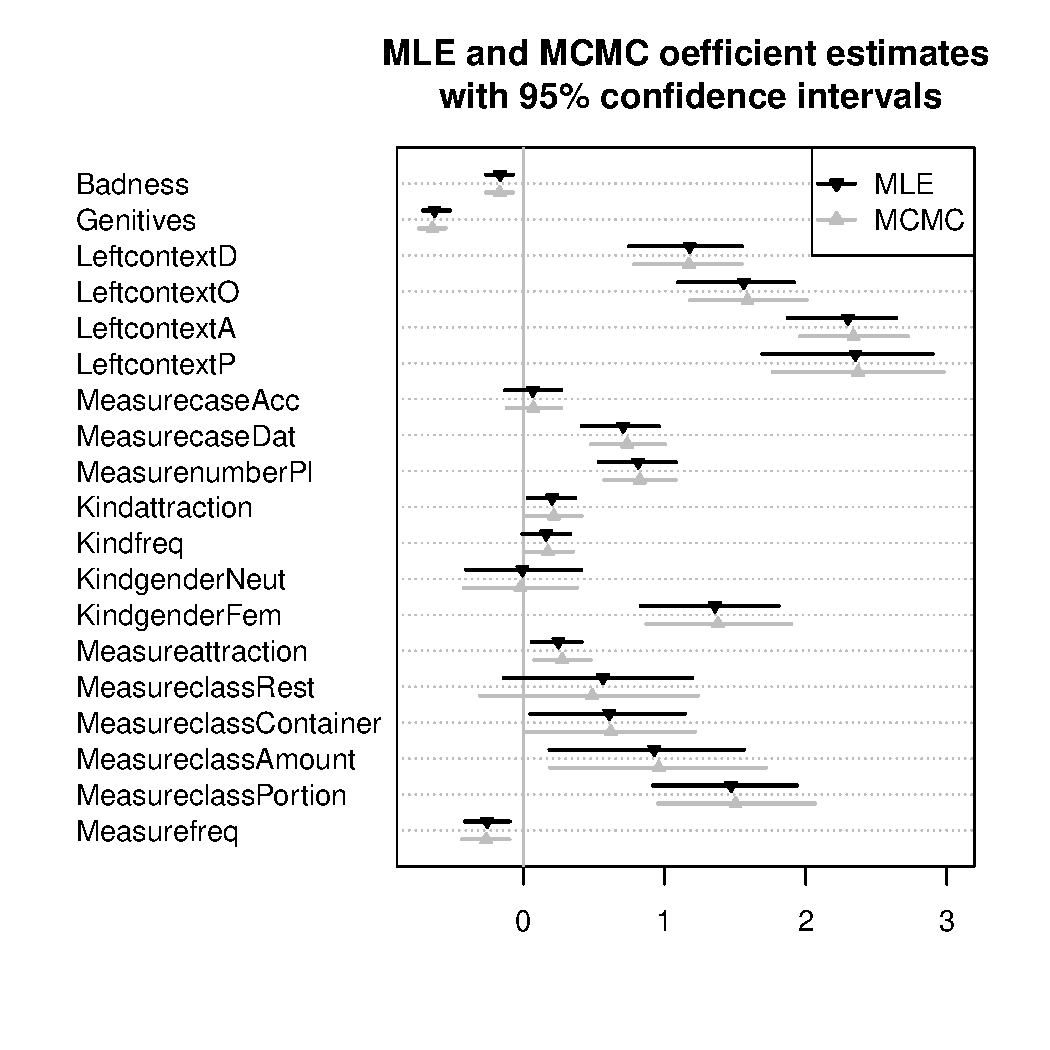
\includegraphics[width=0.85\textwidth]{../R/output/corpus_fixeffs_mle+mcmc}
  \caption{Coefficients (MLE and MCMC) with 95\% confidence intervals (for details see text); the intercept (\textit{Cardinal=Yes}, \textit{Measurecase=Nom}, \textit{Kindgender=Masc}, \textit{Measureclass=Physical}; 0 for all numeric z-transformed regressors) is -4.328 (MLE) and -4.441 (MCMC)}
  \label{fig:fixeffs}
\end{figure}

In this section, I report the results of fitting a multilevel model to the data using R \citep{R}, \textit{lme4} \citep{lme4} for Maximum Likelihood Estimation, and \textit{rstanarm} \citep{rstanarm} for Markov-Chain Monte Carlo estimation (see Section~\ref{sec:rightstatistics}).
The purpose is to model the influence of the regressors specified in Table~\ref{tab:variables} on the probability that either the \PGCa\ is chosen over the \NACa.
All regressors from Table~\ref{tab:variables} were included, and the measure lemma and the kind noun lemma were specified as varying-intercept random effects.
The sample size was $n=5,063$ with $1,1344$ cases of \PGCa\ and $3,929$ cases of \NACa.
The results of the estimation are shown in Table~\ref{tab:bigtable} and in Figure~\ref{fig:fixeffs}.
The regressors with the measure lemma as their unit of reference have no within-measure lemma variance, and the \textit{glmer} function automatically estimates them as \textit{group level predictors} (or \textit{second-level effects}), cf.\ \cite[265--269,302--304]{GelmanHill2006}.
The same goes for those listed with the kind lemma as their unit of reference.
Given the coding of the response variable, coefficients leaning to the positive side can be interpreted as favouring the \PGCa.

\begin{sidewaystable}
  \centering
  \resizebox{\textheight}{!}{
  \begin{tabular}{llrlp{0.5em}rrp{0.5em}rrp{0.5em}rrp{0.5em}cc}
      Level & Regressor & \multicolumn{1}{l}{\pPB} & Level  && \multicolumn{2}{l}{Coefficient} && \multicolumn{2}{l}{CI low} && \multicolumn{2}{l}{CI high} && \multicolumn{2}{l}{CI contains 0} \\
              &                   &       &           && \multicolumn{1}{l}{MLE} & \multicolumn{1}{l}{MCMC} && \multicolumn{1}{l}{MLE} & \multicolumn{1}{l}{MCMC} && \multicolumn{1}{l}{MLE} & \multicolumn{1}{l}{MCMC} && \multicolumn{1}{l}{MLE} & \multicolumn{1}{l}{MCMC} \\\midrule
       First     & Badness           &  0.002 &           && -0.152 & -0.155 && -0.247 & -0.247 && -0.061 & -0.065 && * & * \\
                 & Cardinal          &  0.001 & No        &&  1.189 &  1.222 &&  0.862 &  0.927 &&  1.466 &  1.496 && * & * \\
                 & Genitives         &  0.001 &           && -0.693 & -0.711 && -0.768 & -0.801 && -0.592 & -0.616 && * & * \\
                 & Measurecase       &  0.001 & Acc       &&  0.030 &  0.031 && -0.150 & -0.159 &&  0.212 &  0.222 &&   &   \\
                 &                   &        & Dat       &&  0.705 &  0.729 &&  0.455 &  0.465 &&  0.944 &  0.995 && * & * \\[0.5\baselineskip]
       
       Second    & Kindattraction    &  0.020 &           &&  0.225 &  0.244 &&  0.049 &  0.056 &&  0.393 &  0.422 && * & * \\
       (Kind)    & Kindfreq          &  0.095 &           &&  0.146 &  0.164 && -0.023 & -0.016 &&  0.301 &  0.341 &&   &   \\
                 & Kindgender        &  0.001 & Neut      &&  0.021 &  0.013 && -0.367 & -0.409 &&  0.392 &  0.435 &&   &   \\
                 &                   &        & Fem       &&  1.269 &  1.289 &&  0.800 &  0.788 &&  1.709 &  1.783 && * & * \\[0.5\baselineskip]
       
       Second    & Measureattraction &  0.001 &           &&  0.282 &  0.299 &&  0.106 &  0.102 &&  0.447 &  0.515 && * & * \\
       (Measure) & Measureclass      &  0.001 & Container &&  0.252 &  0.257 && -0.265 & -0.303 &&  0.788 &  0.813 &&   &   \\
                 &                   &        & Rest      &&  0.421 &  0.379 && -0.209 & -0.378 &&  1.063 &  1.091 &&   &   \\
                 &                   &        & Amount    &&  0.831 &  0.889 &&  0.215 &  0.220 &&  1.432 &  1.569 && * & * \\
                 &                   &        & Portion   &&  1.217 &  1.253 &&  0.675 &  0.689 &&  1.684 &  1.840 && * & * \\
                 & Measurefreq       &  0.005 &           && -0.231 & -0.232 && -0.363 & -0.395 && -0.079 & -0.073 && * & * \\

  \end{tabular}
  }
  \caption{Coefficient table comparing Maximum Likelihood Estimation (MLE, with 95\% bootstrap confidence interval) and `Bayesian' Markov-Chain Monte Carlo estimation (MCMC); the intercept (\textit{Cardinal=Yes}, \textit{Measurecase=Nom}, \textit{Kindgender=Masc}, \textit{Measureclass=Physical}; 0 for all numeric z-transformed regressors) is -3.548 (MLE) and -3.700 (MCMC)}
  \label{tab:bigtable}
\end{sidewaystable}


Standard diagnostics for the Maximum Likelihood Estimation (MLE) show that the model quality is quite high.
Generalised variance inflation factors for the regressors were calculated to check for multicollinearity \citep{FoxMonette1992,ZuurEa2010}, and none of the corrected $\text{GVIF}^{1/2\text{df}}$ was higher than $1.6$.
Nakagawa \& Schielzeth's pseudo-coefficient of determination is $R_m^2=0.409$ and $R^2_c=0.495$ (see \citealp{Gries2015} for a linguist-friendly introduction to these $R^2$ measures, or else \citealp{NakagawaSchielzeth2013}).
The rate of correct predictions is $0.843$, which means a proportional reduction of error of $\lambda=0.297$.
The measure lemma intercepts have a standard deviation of $\sigma_{\text{Measurelemma}}=0.448$, the kind lemma intercept $\sigma_{\text{Kindlemma}}=0.604$.

The coefficient estimates are specified in Table~\ref{tab:bigtable} for each regressor (or regressor level) in the columns labelled \textit{Coefficient}.
For a robust quantification of the precision of the estimation, I ran a parametric bootstrap (using the \mbox{\textit{confint.merMod}} function from \textit{lme4}) with $1,000$ replications, and using the percentile method for the calculation of the intervals.
The resulting 95\% bootstrap confidence intervals are reported in Table~\ref{tab:bigtable} in the columns labelled \textit{CI low} and \textit{CI high} (= upper and lower 2.5th percentiles).
The column \textit{CI contains 0} shows an asterisk for those intervals that do \textit{not} include 0.
Furthermore, for each regressor, a $p$ value was obtained by dropping the regressor from the full model, re-estimating the nested model and comparing it to the full model.
Instead of inexact Wald approximations or Likelihood Ratio Tests, I used a drop-in bootstrap replacement for the Likelihood Ratio Test from the function \textit{PBmodcomp} from the \textit{pbkrtest} package \citep{HalekohHojsgaard2014}.
I call the corresponding value $p_{\text{PB}}$, and it is given in the appropriately labeled columns in Table~\ref{tab:bigtable}.
Only \textit{Kindfreq} ($\mpPB=0.095$) can be seen as slightly too high to be convincing (non-significant).

Finally, I show that Bayesian methods in the form of Markov-Chain Monte Carlo estimation do not necessarily (and in this case predictably) lead to different results.
The model was re-estimated using the \textit{stan\_glmer} function from the \textit{rstanarm} package, which provides an \textit{lme4}-compatible syntax for estimating common model types with the \textit{stan} software \citep{CarpenterEa2017}.
The algorithm was run with $4$ chains and $1,000$ iterations, and I used plausible default priors.
Most notably, priors for coefficients were specified as $\mathcal{N}(0,10)$ because coefficients higher than $10$ or lower than $-10$ are extremely rare in well-specified models on appropriate data.%
\footnote{Consider that with a coefficient of $10$, each increase by $1$ in the regressor variable means an increase in odds of $exp(10)=22,026.47$.
To reliably estimate such coefficients, extremely large samples would be required.}
The algorithm converged, and for all coefficients, the $\hat{R}$ diagnostic was exactly $1$.
The resulting coefficients and intervals as well as an * are also given in Table~\ref{tab:bigtable} in the columns labelled \textit{MCMC}.
Both methods lead to exactly the same results (minus negligible numerical differences) as expected given the modest complexity of the model structure and the large sample size (see Section~\ref{sec:rightstatistics}).
The signs and magnitudes of the coefficients are identical, and confidence intervals have the same width and symmetry properties.
Figure~\ref{fig:fixeffs} illustrates this by also showing both estimates.
Since both estimators converge, I only interpret the MLE model in the next section.


%%%%%%%%%%%%%%%%%%%%%%%%%%%%%%%%%%%%%%%%%%%%%%%%%%%%%%%%%%%%%%%%%%%%%%%
%%%%%%%%%%%%%%%%%%%%%%%%%%%%%%%%%%%%%%%%%%%%%%%%%%%%%%%%%%%%%%%%%%%%%%%


\subsection{Interpretation}
\label{sec:interpretation}

% ATTRACTION

\begin{figure}[h!]
  \centering
  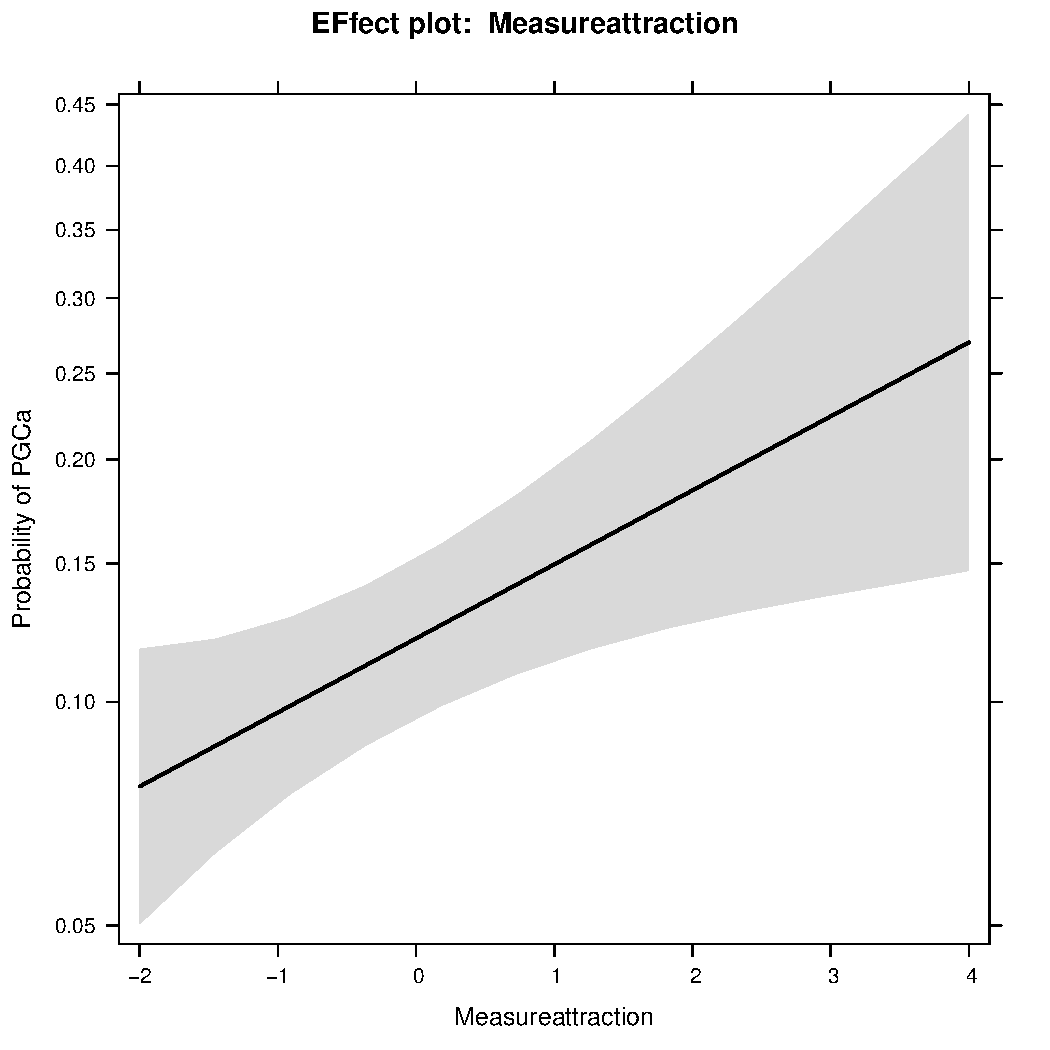
\includegraphics[width=0.5\textwidth]{../R/output/corpus_Measureattraction}~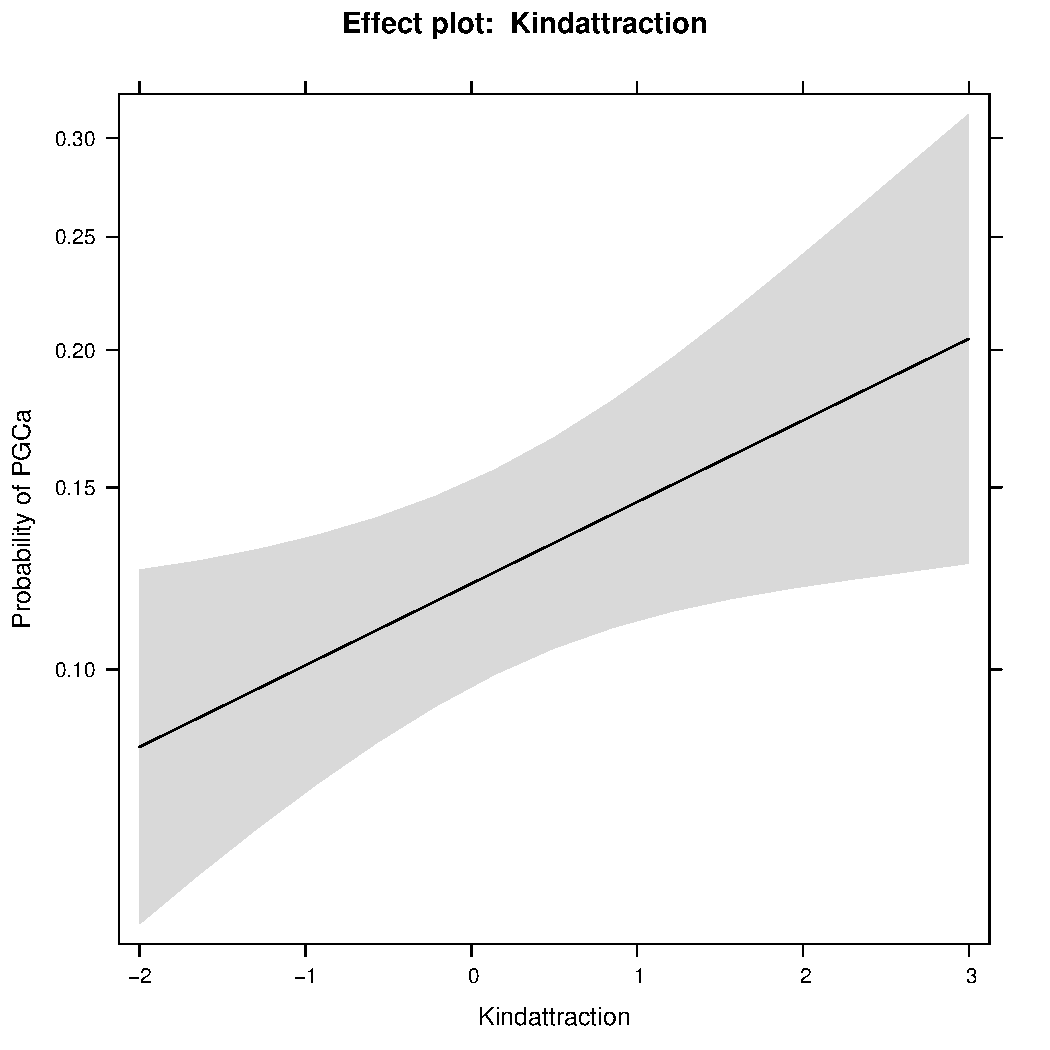
\includegraphics[width=0.5\textwidth]{../R/output/corpus_Kindattraction}
  \caption{Effect plots for the regressors \textit{Measureattraction} and \textit{Kindattraction}; y axes are not aligned}
  \label{fig:eff:attraction}
\end{figure}

The results reported in Section~\ref{sec:corpushierarchicalmodel} generally confirm the hypotheses from Section~\ref{sec:analyses}.
First, the prototypicality effect related to the non-alternating \PGCd\ and \NACb\ can be shown, see the effect plots in Figure~\ref{fig:eff:attraction}.%
\footnote{Effect plots were created using the \textit{effects} package \citep{Fox2003}.
They show the changes in probability for the outcome (y axis) dependent on values of a regressor (x axis), at typical values of all other regressors.}
The effect is mostly as expected:
if a lemma appears relatively more often in the \PGCd\ (compared to its frequency in the \NACb), the more often the \PGCa\ is chosen over the \NACa\ with this specific lemma.
The effect for measure nouns is stronger, and it was estimated with higher precision.

An interesting picture emerges for the lemma frequencies.
A higher than average lemma frequency of measure nouns favours the \NACa\ ($\beta_{\text{Measurefreq}}=-0.231$, $\mpPB=0.005$) as expected if we assume at least a tendency for highly grammaticalised items to be more frequent.
With kind nouns, higher frequency seems to favour the \PGCa ($\beta_{\text{Kindfreq}}=0.146$, $\mpPB=0.095$).
However, there is no clear theoretical interpretation (see Section~\ref{sec:analyses}), and the estimate is imprecise (not significant at $\alpha=0.05$, see above).
The effect can therefore be ignored or treated as a nuisance variable.


% GRAMMATICALISATION
% => lemmas and lemma classes

\begin{figure}[h!]
  \centering
  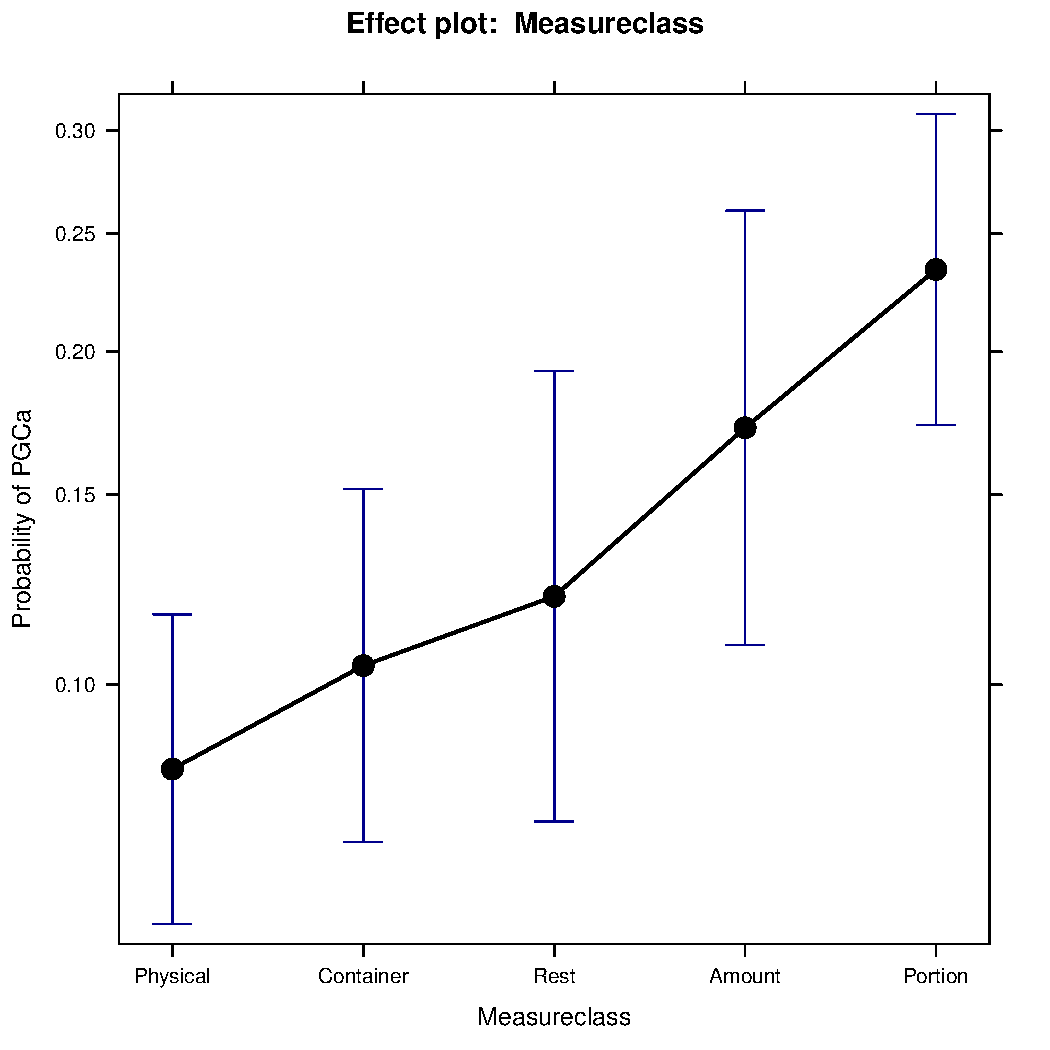
\includegraphics[width=0.75\textwidth]{../R/output/corpus_Measureclass}
  \caption{Effect plot for the regressor \textit{Measureclass}}
  \label{fig:eff:measureattraction}
\end{figure}

In Section~\ref{sec:analyses}, it was also hypothesised that classes of measure nouns with a higher degree of grammaticalisation should favour the \PGCa.
The \textit{Measureclass} second-level predictor was successfully estimated ($\mpPB=0.001$).
Looking at the effect plot in Figure~\ref{fig:eff:measureattraction}, it is evident that abstract non-referential physical measure nouns (such as \textit{Gramm} `gram' or \textit{Liter} `litre') with a high degree of grammaticalisation favour the \NACa.
At the other end of the scale, nouns denoting natural portions like \textit{Haufen} `heap', \textit{Bündel} `bundle', \textit{Schluck} `gulp' favour the \PGCa.
These are referential nouns, confirming the hypothesis that it is prototypical of the PGC to contain two referential nouns, while the NAC only contains one (the kind noun).

% CARDINALS

\begin{figure}[h!]
  \centering
  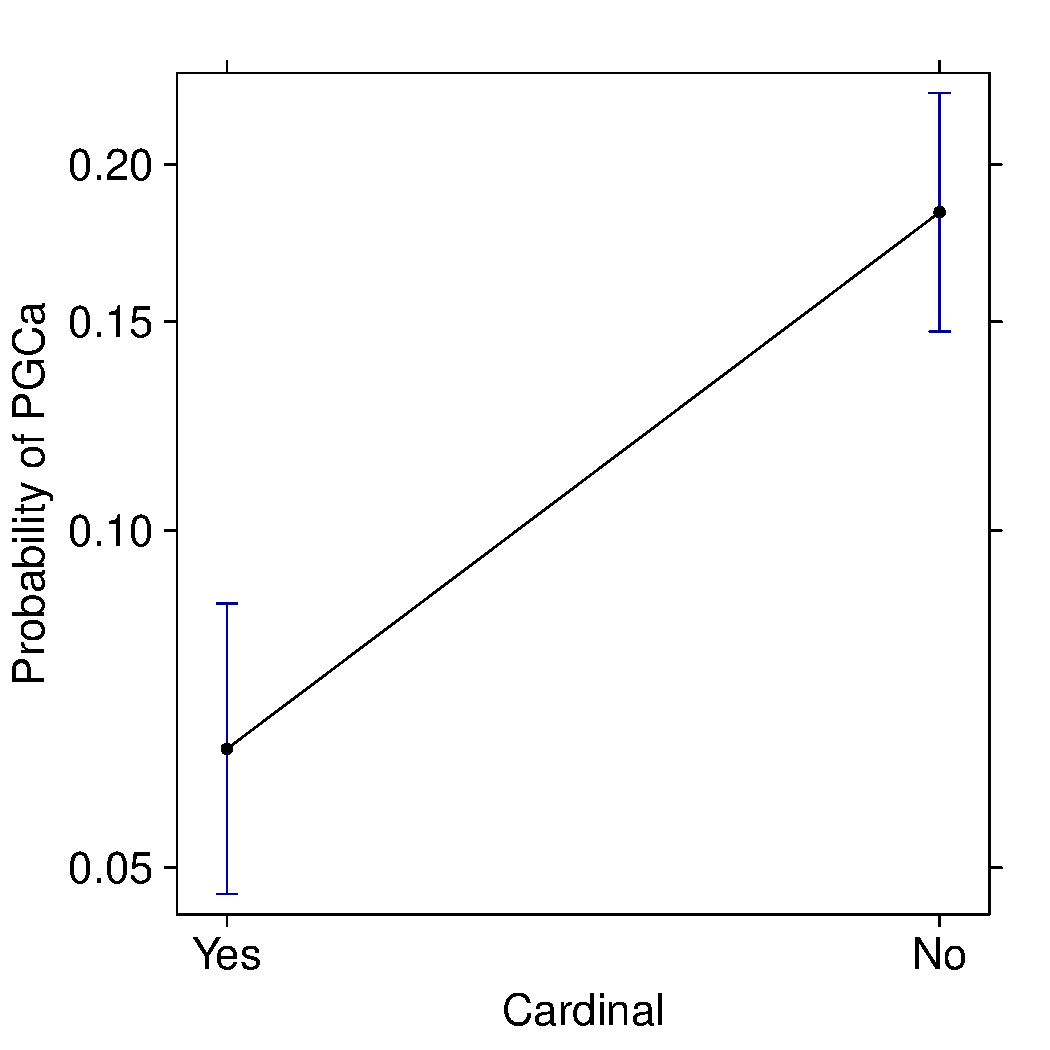
\includegraphics[width=0.75\textwidth]{../R/output/corpus_Cardinal}
  \caption{Effect plot for the regressor \textit{Cardinal}}
  \label{fig:eff:leftcontext}
\end{figure}

I now turn to the predicted effect of cardinals as modifiers of the measure noun.
Figure~\ref{fig:eff:leftcontext} shows that cardinals indeed influence the choice of the variant ($\mpPB=0.001$), and that cardinals have a strong tendency to co-occur with the \NACa.
This effect was predicted in Section~\ref{sec:analyses}.

% REGISTER
% => Badness
% => Genitives

The register-related proxy variables point into the expected direction.
Increased \textit{Badness} of the document favours the \NACa\ ($\beta_{\text{Badness}}=-0.152$, $\mpPB=0.002$), and so does a lesser density of genitives ($\beta=-0.693$, $\mpPB=0.001$).
While these are poor proxies to register (and partially circular in the case of \textit{Genitives}), this result can at least encourage future work into register effects. 

% NUISANCE
% => dative effect
% => frequency

The influence of \textit{Measurecase} ($\mpPB=0.001$) is as predicted in previous analyses (see Section~\ref{sec:analyses}).
A measure noun in the dative favours the \PGCa\ with $\beta_{\text{MeasurecaseDat}}=0.705$ (compared to the nominative, which is on the intercept).
Although \textit{Measurecase} is a nuisance variable in the context of this study, convergence with previous work strengthens its validity.

%%%%%%%%%%%%%%%%%%%%%%%%%%%%%%%%%%%%%%%%%%%%%%%%%%%%%%%%%%%%%%%%%%%%%%%
%%%%%%%%%%%%%%%%%%%%%%%%%%%%%%%%%%%%%%%%%%%%%%%%%%%%%%%%%%%%%%%%%%%%%%%
%%%%%%%%%%%%%%%%%%%%%%%%%%%%%%%%%%%%%%%%%%%%%%%%%%%%%%%%%%%%%%%%%%%%%%%


\section{Correlating corpus findings with experiments}
\label{sec:experimental}

\subsection{Experiment 1: forced-choice}
\label{sec:exp:fc}

In the two experiments reported in this section, I use probabilities for the alternating constructions calculated for attested material, and I correlate these probabilities with the participants' reactions.
Thus, a direct link can be established between output material found in corpora and the behaviour of linguistic agents (see also Section~\ref{sec:cogocl}).
Both experiments use sentences containing attested MNPs from the corpus sample (embedded into simplified sentences) as stimuli.
Also, the probabilities that the corpus-based model assigns to the two variants in these sentences is used as the main regressor in both studies.

The first experiment tests preferences for constructions explicitly.
\cite{FordBresnan2013} use the \textit{split-100} task in which participants have to distribute $100$ points between the alternatives, assigning more points to more natural sounding alternative.
In essence, participants distribute a probability mass between two variants, which is intended to produce more subtle results compared to a two-alternative forced-choice task \cite{Rosenbach2013}, where participants have to choose one of two variants.
The split-100 paradigm has been criticised in \cite{ArppeJaervikivi2007}.
The criticism was reiterated in \cite{DivjakEa2016}, where they use a forced-choice task.
In \cite{VerhoevenTemme2017}, it was shown that results from forced-choice and split-100 experiments mostly converge, which is expected in the long run if a probability is turned into a binary decision.
I present a forced-choice experiment in Section~\ref{sec:exp:fc} and not a split-100 experiment, mainly because in a dry-run of the experiment, participants complained about the unnaturalness of the task of distributing a probability mass across two variants.
Participants had to chose between two sentences differing only in that one contained the \NACa\ and the other contained the \PGCa.
The analysis compares the probabilities assigned to stimuli by the corpus-derived model with the frequency with which participants chose the variants for the same stimuli.

There were 24 participants (native speakers of German without reading or writing disabilities) aged 19 to 30 living permanently in [name of city anonymised], who were recruited from introductory linguistics courses at [name of university anonymised].
Although the experiment was conducted in the last four weeks of their first semester, participants had no deeper explicit knowledge of linguistics, grammar, or experimental methods.
None of them had ever participated in a forced-choice experiment before.
Participation was voluntary, but participants received credit in partial fulfillment of course requirements.

As stimuli, attested MNPs from the corpus study were used, but the sentences were radically simplified to avoid influences from contextual nuisance variables as much as possible.
The approach is also justified because according to the theoretical assessment in Section~\ref{sec:analyses}, the choice of variants depends mostly on a very local constructional context.
I sampled 16 MNPs from the corpus, and it was made sure that the simplifications and normalisations did not affect any of the regressors used in the corpus study.
In the simplified sentences, the case, number, etc. of the MNP remained the same as in the attested sentence, as well as the choice of lexical material within the MNP.
Eight sentences contained masculine or neuter kind nouns, the other eight contained feminine kind nouns.
Furthermore, in each of the masculine\slash neuter and feminine groups, four sentences originally containing the \NACa\ and four sentences originally containing the \PGCa\ were chosen.
More precisely, the sentences were sampled as \textit{highly prototypical examples} of \PGCa\ (high probability assigned by GLMM) and \NACa\ (low probability assigned by GLMM), respectively.%
\footnote{Remember from Section~\ref{sec:corpusstudies} that the model predicts the probability that the \PGCa\ is chosen over the \NACa.}
High and low probability were defined as the top and bottom 20\% of all probabilities assigned by the GLMM.
Lemmas and feature combinations were made unique within each group whenever possible.
The design is summarised in Table \ref{tab:experiment1:design}.

\begin{table}
  \centering
  \begin{tabular}[h]{rcc}
     & Masculine\slash Neuter & Feminine \\
     \midrule
     \textbf{high prob.\ for PGC\Subsf{adj}} & 4 sentences\Supsf{a} & 4 sentences\Supsf{a} \\
     \textbf{low prob.\ for PGC\Subsf{adj}} & 4 sentences\Supsf{a} & 4 sentences\Supsf{a} \\
  \end{tabular}
  \caption{The four groups of sentences chosen as stimuli (\Supsf{a}Among the 4 sentences, combinations of important factor values were made unique whenever possible.)}
  \label{tab:experiment1:design}
\end{table}

The pairs of stimuli were the sentence containing the preferred construction (according to the corpus GLMM) and a modified version containing the dispreferred construction.
They were presented next to each other, and a 20 second time limit for each choice was set.%
\footnote{No participant ever exceeded the time limit.}
The position on the screen (left\slash right) and the order of sentences were randomised for each participant.
As fillers, 23 pairs of sentences exemplifying similar alternation phenomena from German morpho-syntax were used.
Thus, participants saw 39 pairs of sentences and 78 sentences in total.
They were instructed to select from each pair of sentences the one that seemed more natural to them in the sense that they would use it rather than the other one.
The experiment was conducted using \textit{PsychoPy} \citep{Peirce2007}.

\begin{figure}[hb!]
\centering
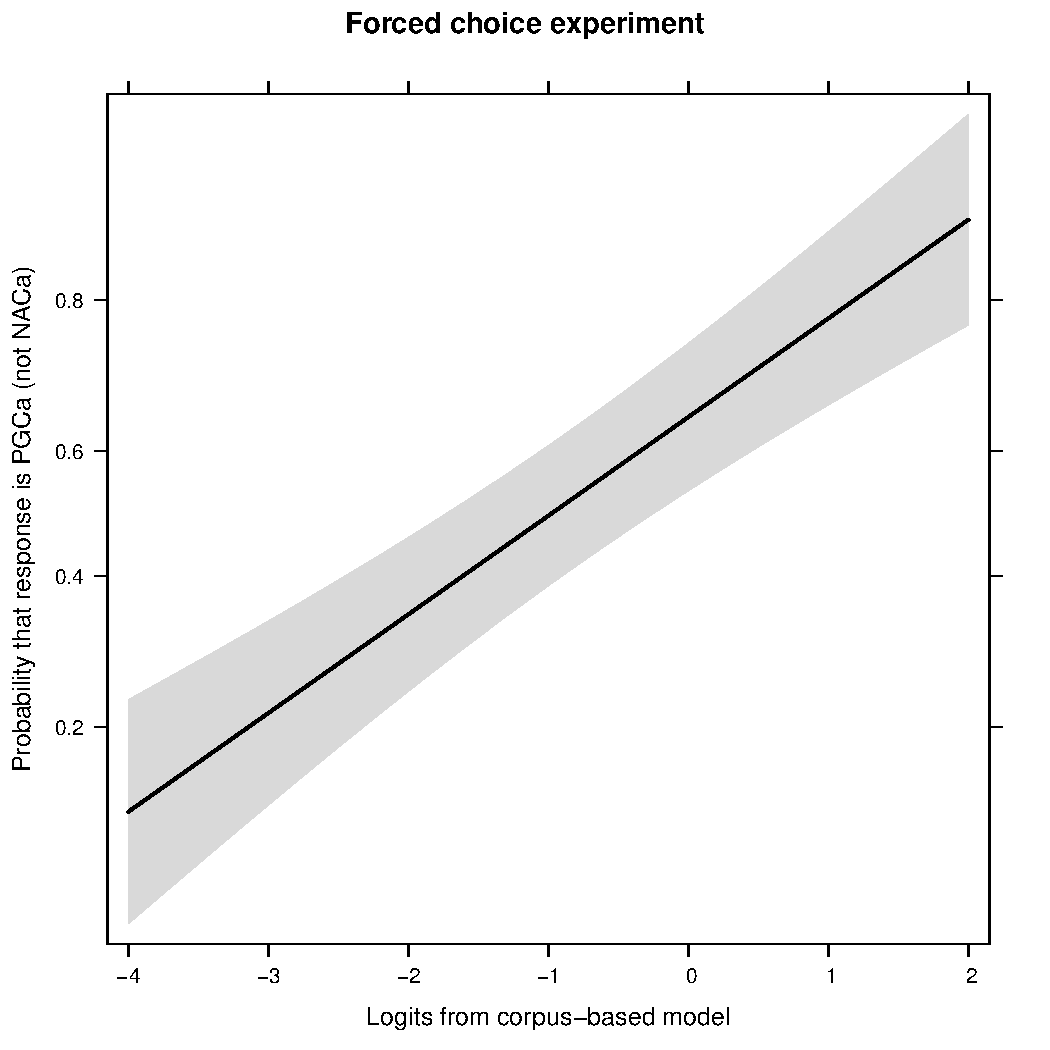
\includegraphics[width=0.75\textwidth]{../R/output/fc_effects}
\caption{Effect plot for the multilevel logistic regression in the forced-choice experiment: predictability of participants' choices using the probabilities derived from the corpus-based GLMM}
\label{fig:afc:effects}
\end{figure}

Then, a multilevel logistic regression was specified with the probability of the \PGCa\ predicted for each sentence by the corpus-based GLMM as the only fixed effect \textit{Modelprediction}.%
\footnote{The document-level variables \textit{Badness} and \textit{Genitives} were set to $0$, which is the mean for z-transformed variables.}
A random intercept and slope were added for the individual sentence (item) in order to catch idiosyncrasies of single sentences.
Also, a random intercept and slope for participants was added.%
\footnote{The random slopes were added to comply with \citet[257]{BarrEa2013} who predict \textit{catastrophically high Type I error rates} for experimental designs with within-subject manipulations if random effects structures are not kept maximal.
Notice that the model reported here was estimated with conceptually identical results with regard to the predictor of interest (\textit{Modelprediction}) if only random intercepts were used.}
Coefficients were estimated with Maximum Likelihood Estimation (\textit{lmer} function from \textit{lme4}).
The number of observations was $n=384$.

A certain amount of the variance can be accounted for by idiosyncrasies of single sentences ($\sigma_{\text{Sentence}}=1.785$, $\sigma^{\text{Modelprediction}}_{\text{Sentence}}=5.996$, $16$ levels).%
\footnote{I use $\sigma^f_r$ to denote the standard deviation of the of the random intercepts for the fixed effect $f$ varying by random effect $r$.}
Also, among participants, there are clearly different preferences ($\sigma_{\text{Participant}}=0.781$, $\sigma^{\text{Modelprediction}}_{\text{Participant}}=0.484$, $24$ levels).
On the extreme sides, one participant chose the \PGCa\ in $13$ of $16$ cases, and two participants only chose it in $5$ of $16$ cases.
The regressor \textit{Modelprediction} achieves $\mpPB=0.007$ ($1,000$ replications) and is estimated at $5.408$ relative to an intercept of $-1.304$.
The confidence interval from a parametric bootstrap ($1,000$ replications, percentile method) for the regressor is acceptable but slightly large with a lower bound of $1.626$ and an upper bound of $8.397$.
Nakagawa \& Schielzeth's pseudo-coefficients of determination are $R^2_{m}=0.227$ and $R^2_{c}=0.561$, which means that over 22\% of the variance in the data can be explained by considering only the predictions from the corpus-based GLMM.
The effect display for the single fixed regressor \textit{Modelprediction} is given in Figure \ref{fig:afc:effects}.
The result is very clear.
The higher the probability of the \PGCa\ predicted from usage-data, the more often participants chose the \PGCa\ variant in the forced-choice task.
In summary, the forced-choice experiment clearly succeeded in corroborating the results from the corpus study in as much as the preferences extracted from usage data correspond to native speakers' choices.


%%%%%%%%%%%%%%%%%%%%%%%%%%%%%%%%%%%%%%%%%%%%%%%%%%%%%%%%%%%%%%%%%%%%%%%
%%%%%%%%%%%%%%%%%%%%%%%%%%%%%%%%%%%%%%%%%%%%%%%%%%%%%%%%%%%%%%%%%%%%%%%

\subsection{Experiment 2: self-paced reading}
\label{sec:exp:spr}

The second experiment tests preferences more implicitly.
It is expected that reading less prototypical variants (the one assigned a low probability by the corpus-derived model) in a given context and with given lexical material incurs a processing overhead for the reader (\citealp{Kaiser2013}).
In Section~\ref{sec:exp:spr}, a self-paced reading experiment is therefore presented.
In a very similar fashion, \cite{DivjakEa2016} apply the self-paced reading paradigm in the validation of corpus-based models.
The analysis compares the corpus-derived probabilities with potential lags in reading time for sentences with the preferred and the non-preferred constructions.

Conretely, the exact same stimuli as in the forced-choice experiments were used.
Each participant read both the $16$ sentences with the variant predicted by the corpus model and the $16$ modified sentences with the variant that the corpus model does not predict.%
\footnote{Notice that lemmas and their frequencies as well as lemma classes are included as regressors in the corpus-based GLMM, and there was consequently no additional controlling of lemma frequencies, etc.}
To minimise repetition effects, the stimuli for each participant were separated into two blocks of $16$ targets and $33$ fillers per block.
In the experiment, participants first read all sentences from the first block, then all sentences from the second block.
It was made sure that from each target sentence pair, one sentence was assigned to the first block, and the other sentence to the other block.
The assignment of members of the individual sentence pairs to the blocks was randomised for each participant individually, and so was the order within each block.
The sentences from each pair of variants were kept as far apart as possible.
The fillers also came in pairs such that the second block exclusively contained sentences to which participants had been exposed in the first block in slightly modified form.
In total, each participant read $98$ sentences.
After each sentence, participants had to answer simple (non-metalinguistic) yes-no questions about the previous sentence as distractors.
The distractor questions were different ones in the first and the second block.
There were $38$ (different) participants recruited in exactly the same manner as for the experiment reported in Section~\ref{sec:exp:fc}.
None of them had ever participated in any kind of reading experiment, and none of them took part in the first experiment (and vice versa).
The experiment was conducted using \textit{PsychoPy}.

The reading times were residualised per speaker based on the reading times of all words (not just the targets) by that speaker.
The adjective and the kind noun (\ie\ the constituents bearing the critical case markers) were used as the target region, such as the bracketed words in the example \textit{zwei Gläser} [\textit{sprudelndes Wasser}] `two glasses of sparkling water'.
Outliers farther than 2 inter-quartile ranges from the mean logarithmised residual time were removed ($64$ data points), resulting in a total number of $n=1,152$ observations.
An LMM was specified with the logarithmised residual reading times as the response variable, and the probabilities derived from the corpus GLMM (\textit{Modelprediction}) as the main regressor.
Since the corpus GLMM predicts the probability of the \PGCa\ (vis-à-vis the \NACa), it is expected that reading times are positively correlated (longer reading times) with the probability if the stimulus actually contains the \NACa, and negatively correlated (shorter reading times) if the stimulus actually contains the \PGCa.
To account for this, an interaction between \textit{Modelprediction} and \textit{Construction} (levels \textit{PGCa} and \textit{NACa}) was added to the model.
Furthermore, the position ($1$--$98$) of the sentence in the individual experiment (\textit{Position} was included as a fixed effect to control for increasing reading speed during experiment runs.
Random intercepts were specified for \textit{Participant} and \textit{Item} (the $16$ sentence pairs are one \textit{Item} each).%
\footnote{I tried random slopes in order to keep the random effect structure maximal \citep{BarrEa2013}, but it was impossible to get the algorithm to converge due to the added complexity of the interaction.}

\begin{table}
  \centering
  \begin{tabular}{lrrrc}
    Regressor & \multicolumn{1}{r}{Coefficient} & \multicolumn{1}{r}{CI low} & \multicolumn{1}{r}{CI high} & \multicolumn{1}{r}{0 in CI} \\ \midrule
    ConstructionPGCa                 &  0.054 &  0.012 &  0.095 &  *  \\ 
    Modelprediction                  & -0.006 & -0.113 &  0.110 &     \\ 
    Position                         & -0.005 & -0.005 &  0.004 &     \\ 
    ConstructionPGCa:Modelprediction & -0.125 & -0.234 & -0.023 &  *  \\ 
  \end{tabular}
  \caption{Fixed effect coefficient table for the LMM used to analyse the self-paced reading experiment; the intercept is 0.829}
  \label{tab:exp:spr}
\end{table}

Table~\ref{tab:exp:spr} shows the coefficient estimates with a 95\% parametric bootstrap confidence interval ($1,000$ replications, percentile method).
The standard deviation of the participant intercepts is $\sigma_{\text{Participant}}=0.079$ and of the item intercepts $\sigma_{\text{Item}}=0.037$.
Comparing the full model to a model without the main regressor \textit{Modelprediction} (and consequently also without the interaction with \textit{Construction}) in a PB test gives $\mpPB=0.036$.
Nakagawa and Schielzeth's pseudo-determination coefficients are $R^2_m=0.237$ and $R^2_c=0.346$.

\begin{figure}[h]
\centering
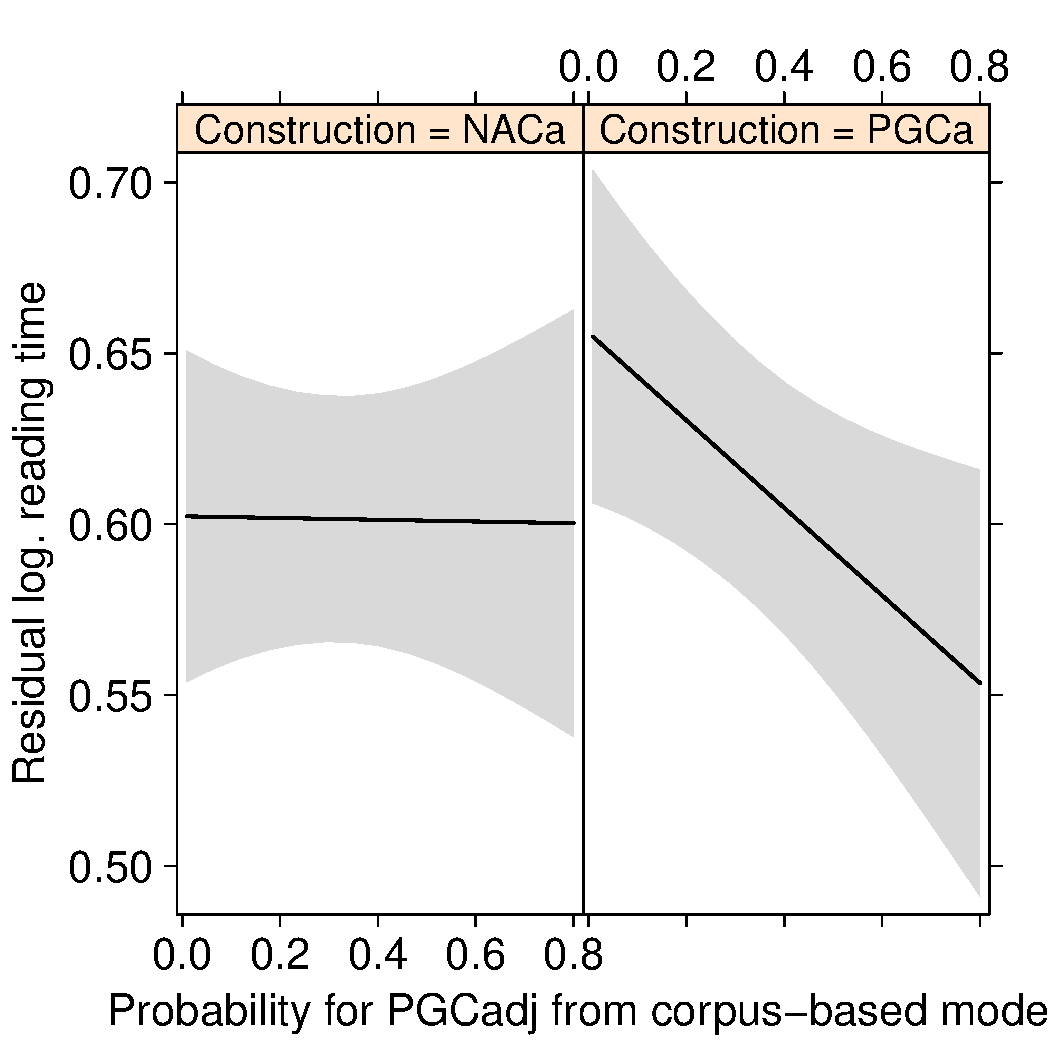
\includegraphics[width=0.75\textwidth]{../R/output/spr_effects}
\caption{Effect plot for the LMM in the self-paced reading experiment: modeling participants' residualised log reading times on the probabilities given by the corpus-based GLMM}
\label{fig:spr:effects}
\end{figure}

The overall model quality is thus good, and the effect plot for the main effect is shown in Figure~\ref{fig:spr:effects}.
The estimate for the sentences with \NACa\ is obviously imprecise, and no differences in reading times are observed.
There is a clearer effect in the sentences with \PGCa, which is also confirmed by the significant results from the bootstrapped confidence intervals (see Table~\ref{tab:exp:spr}) and from the PB test reported above.
The \PGCa\ brings about an increased reading time ($\beta_{\text{ConstructionPGCa}}=0.054$), which is plausible because it is the much rarer construction (see Section~\ref{sec:corpusstudies}).
However, if it occurs in a prototypical context and with prototypical lexical material, reading times drop ($\beta_{\text{ConstructionPGCa:Modelprediction}}=-0.125$).
This can be seen in the downward slope in the right panel of Figure~\ref{fig:spr:effects}.
This fits into the general picture in as much as the construction with the lower frequency might be developing towards a more sharply defined prototype.%
\footnote{In this context, it should be remembered from Section~\ref{sec:gettingdata} that even the \PGCd\ is much rarer that the \NACb\ ($17,252$ vs.\ $315,635$ occurrences in the auxiliary corpus samples).}
Conversely, the \NACa\ (like the NAC in general) might be the highly frequent default which does not incur reading time penalty, even if it is not the optimal choice in the given context and with the given lexical material.

This concludes the report of the two experiments.
In the final section, I take stock and summarise the contribution of the present study to the research on alternations in cognitive linguistics.


%%%%%%%%%%%%%%%%%%%%%%%%%%%%%%%%%%%%%%%%%%%%%%%%%%%%%%%%%%%%%%%%%%%%%%%
%%%%%%%%%%%%%%%%%%%%%%%%%%%%%%%%%%%%%%%%%%%%%%%%%%%%%%%%%%%%%%%%%%%%%%%
%%%%%%%%%%%%%%%%%%%%%%%%%%%%%%%%%%%%%%%%%%%%%%%%%%%%%%%%%%%%%%%%%%%%%%%


\section{Conclusions}
\label{sec:conclusion}

This paper stands in a now ten year-old tradition of research on grammatical alternations using corpus and experimental data.
In my view, the main tenets of this line of research are:
(i)~Language, viewed from a cognitively realistic angle, is a probabilistic phenomenon and cannot be modeled appropriately within Aristotelian frameworks that assume discrete categories.
(ii)~Corpora are collections of usage events (language production) and can therefore be used to evaluate both the claim made in (i) and specific theoretical claims (in case studies) about factors influencing speakers' decisions to use specific forms or constructions.
(iii)~Given (ii), we expect results from corpus analyses and from appropriate experiments to yield similar results, not necessarily as a form of validation of the corpus-based findings, but as converging evidence.
I consider these three points to be of utmost importance because they clearly set this brand of cognitive linguistics apart from \textit{both} Aristotelian frameworks of the generative flavour \textit{and} introspective, non-empirical, and anti-quantitative versions of cognitive linguistics (see \citealp{Dabrowska2016} for an impressive philippic against such approaches).

The present paper adds to the evidence that all of the aforementioned three points are correct.
A grammatical alternation in German measure NPs was examined using corpus data based on factors partly derived from existing accounts, formulated in terms of construction prototypes.
The preferences extracted from the DECOW web corpus were confirmed in a forced-choice experiment, in which participants explicitly chose variants in line with the corpus-derived model.
In a more implicit self-paced reading experiment, it was shown that the much rarer variant brings about a reading time penalty except in cases for which the corpus model predicts very high probability for this variant.

Future work could extend these results and provide a general picture of the constructions expressing measurements (see Section~\ref{sec:descriptive}).
This would be a much more complicated task given that the choices then would no longer be binary, and that the meaning of the alternative ways of expressing measurements are semantically more varied.
Finally, I want to point out that German is mildly under-researched in the specific framework used here.
This is quite surprising given the fact that German morpho-syntax is famous for its alternations, which are usually called \textit{Zweifelsfälle} (`cases of doubt') in the traditional literature \citep{Klein2009}.
Instead of being drowned in normative, descriptive, or didactic discussions, they could serve as ideal test cases in cognitive linguistics.


%%%%%%%%%%%%%%%%%%%%%%%%%%%%%%%%%%%%%%%%%%%%%%%%%%%%%%%%%%%%%%%%%%%%%%%
%%%%%%%%%%%%%%%%%%%%%%%%%%%%%%%%%%%%%%%%%%%%%%%%%%%%%%%%%%%%%%%%%%%%%%%
%%%%%%%%%%%%%%%%%%%%%%%%%%%%%%%%%%%%%%%%%%%%%%%%%%%%%%%%%%%%%%%%%%%%%%%
%%%%%%%%%%%%%%%%%%%%%%%%%%%%%%%%%%%%%%%%%%%%%%%%%%%%%%%%%%%%%%%%%%%%%%%



% \begin{acknowledgement}
%   I want to thank (in alphabetical order) Felix Bildhauer, Samuel Reichert, and Ulrike Sayatz for discussions on relevant aspects of this paper.
%   I also thank Ulrike Sayatz for helping to recruit the participants for the experiments.
%   I am grateful to Kim Maser for her work on the annotation of the concordances.
%   The research presented here was made possible in part through funding from the \textit{Deutsche Forschungsgemeinschaft} (DFG, personal grant SCHA1916/1-1).
% \end{acknowledgement}



%%%%%%%%%%%%%%%%%%%%%%%%%%%%%%%%%%%%%%%%%%%%%%%%%%%%%%%%%%%%%%%%%%%%%%%
%%%%%%%%%%%%%%%%%%%%%%%%%%%%%%%%%%%%%%%%%%%%%%%%%%%%%%%%%%%%%%%%%%%%%%%
%%%%%%%%%%%%%%%%%%%%%%%%%%%%%%%%%%%%%%%%%%%%%%%%%%%%%%%%%%%%%%%%%%%%%%%
%%%%%%%%%%%%%%%%%%%%%%%%%%%%%%%%%%%%%%%%%%%%%%%%%%%%%%%%%%%%%%%%%%%%%%%


\bibliography{rs,cow}
\end{document}

